\documentclass[fontsize=8pt]{scrartcl}
\usepackage[landscape]{geometry}
\usepackage{upgreek}
\usepackage{url}
\usepackage{multicol}
\usepackage{amsmath}
\usepackage{esint}
\usepackage{amsfonts}
\usepackage{tikz}
\usetikzlibrary{decorations.pathmorphing}
\usepackage{amsmath,amssymb}
\usepackage{xstring}		% Für Stringvergleiche und weiteres

\usepackage{colortbl}
\usepackage{xcolor}
\usepackage{mathtools}
\usepackage{amsmath,amssymb}
\usepackage{enumitem}
\usepackage{siunitx}
\usepackage{nicefrac}


\makeatletter

\newcommand*\bigcdot{\mathpalette\bigcdot@{.5}}
\newcommand*\bigcdot@[2]{\mathbin{\vcenter{\hbox{\scalebox{#2}{$\m@th#1\bullet$}}}}}
%		Neue Kommandos, immer in newcommandslist eintragen

% Einstellungen:


% Neue Spaltendefinitionen für Tabellen
\newcolumntype{v}[1]{>{\raggedright\hspace{0pt}}p{#1}}
\newcolumntype{w}[1]{>{\raggedleft\hspace{0pt}}p{#1}}


% % % % % % % % % % % % % % % % % % %
% neue Befehle

% Fließtext

\newcommand{\zB}{\mbox{z.\,B.}\xspace}
\newcommand{\dht}{\mbox{d.\,h.}\xspace}
\newcommand{\oae}{\mbox{o.\,ä.}\xspace}
\newcommand{\oBdA}{\mbox{o.\,B.\,d.\,A.}\xspace}
\newcommand{\idR}{\mbox{i.\,d.\,R.}\xspace}
\newcommand{\RWA}{RWA\xspace}
\newcommand{\horizline}{\rule{1.0\linewidth}{0.4pt}}
\newcommand{\eigenname}[1]{\textsc{#1}}
\newcommand{\figref}[2][S]{\IfStrEq{#1}{S}{Bild~\ref{#2}}	% Singular, ein Bild
						{\IfStrEq{#1}{P}{Bilder~\ref{#2}}	% Plural, mehrere Bilder
						{\errmessage{Option nicht bekannt}}}}	% Fehler
\newcommand{\tabref}[2][S]{\IfStrEq{#1}{S}{Tabelle~\ref{#2}}	% Singular, eine Tabelle
						{\IfStrEq{#1}{P}{Tabellen~\ref{#2}}		% Plural, mehrere Tabellen
						{\errmessage{Option nicht bekannt}}}}	% Fehler
\newcommand{\eqaref}[2][S]{\IfStrEq{#1}{S}{Gleichung~\eqref{#2}}	% Singular, eine Gleichung
						{\IfStrEq{#1}{P}{Gleichungen~\eqref{#2}}	% Plural, mehrere Gleichungen
						{\errmessage{Option nicht bekannt}}}}	% Fehler

\newcommand{\auswahl}[3]{\ifthenelse{\boolean{#1}}{#2}{#3}}


% % % % % % % % % % % % % % % % % % %
% Mathemodus

%\catcode`\_=13 \gdef_#1{\sb{\mathrm{#1}}}	% Indizes global Aufrecht stellen, dies hat auch den Effekt, dass man den _ nur für den Index verwenden kann, da sonst ein Fehler auftritt

\newcommand{\const}{\ensuremath{\mathrm{const.}}}
\newcommand{\pointspace}{\ensuremath{\,}}				    % Abstand hinter Gleichungen
\newcommand{\pointspacek}{\ensuremath{\,\textrm{,}}}       	% dito mit Komma 
\newcommand{\pointspacep}{\ensuremath{\,\textrm{.}}}       	% dito mit Punkt


\newcommand{\upd}{\ensuremath{\mathrm{d}}}					% aufrechtes d
\renewcommand{\d}{\partial\mspace{2mu}} 					% partielle Ableitung (delta)
\newcommand{\intnach}[1]{\, \upd #1}						% Integration nach ...
\newcommand{\komplex}{\ensuremath{\mathrm{j}}}				% imaginäre Einheit
\newcommand{\euler}{\ensuremath{\mathrm{e}}}				% eulersche Zahl

\newcommand{\normal}[1][ ]{\ensuremath{^{n_\mathrm{#1}}}}						% Normalkomponente
\newcommand{\tangential}[1][ ]{\ensuremath{^{t_\mathrm{#1}}}}					% Tangetialkomponente

% mathematische Operatoren

\newcommand{\divergenz}{\ensuremath{\mathrm{div}\,}}
\newcommand{\rotation}{\ensuremath{\mathrm{rot}\,}}
\newcommand{\gradient}{\ensuremath{\mathrm{grad}\,}}
\newcommand{\laplace}{\ensuremath{\Updelta}}

\newcommand{\ehoch}[1]{\ensuremath{\exp \left( #1 \right)}}
\newcommand{\imaginaer}[1]{\ensuremath{\mathfrak{Im} \left\{ #1 \right\}}}
\newcommand{\real}[1]{\ensuremath{\mathfrak{Re} \left\{ #1 \right\}}}

\newcommand{\istgleich}{\ensuremath{\stackrel{!}{=}\,}}
\newcommand{\entspricht}{\ensuremath{\hat{=}\,}}

\newcommand{\mittelwert}[1]{\ensuremath{\left\langle #1 \right\rangle}}
\newcommand{\abs}[1]{\ensuremath{\left| #1 \right|}}

\newcommand{\durchvierpie}[1][1]{\ensuremath{\dfrac{ #1 }{4 \uppi\: \varepsilon_0}}}
\newcommand{\durchzweipie}[1][1]{\ensuremath{\dfrac{ #1 }{2 \uppi\: \varepsilon_0}}}

% mathematische Zahlenbereiche

\newcommand{\IN}{\ensuremath{\mathbb{N}}}			% natürliche Zahlen
\newcommand{\IZ}{\ensuremath{\mathbb{Z}}}			% ganze Zahlen
\newcommand{\IQ}{\ensuremath{\mathbb{Q}}}			% rationale Zahlen
\newcommand{\IR}{\ensuremath{\mathbb{R}}}			% reelle Zahlen
\newcommand{\IC}{\ensuremath{\mathbb{C}}}			% komplexe Zahlen

% Tabellen
\newcommand{\auslassungc}{\multicolumn{1}{c}{---}}
\newcommand{\auslassungl}{\multicolumn{1}{l}{---}}


% Farbbeispiel
\newcommand{\farbbeispiel}[1]{\tikz \filldraw [fill=#1] (0ex,0ex) rectangle (4ex,1.5ex); #1}



% % % % % % % % % % % % % % % % % % %
%	Zeichen



\newcommand{\ergo}{ %		Runder Ergo-Pfeil
	\tikz[baseline]{
		\draw[-latex] (0,0.5ex) .. controls (0.3em,1.4ex) and (0.6em,1.4ex) .. (1.1em,0.5ex);}\;\xspace%
}


\newcommand{\circled}[1]{%	Einkreisen von Zeichen
	\tikz[baseline=(char.base)]{
		\node[shape=circle,draw,inner sep=1.5pt] (char) {#1};} %
}

\newcommand{\transformation}{\mbox{\setlength{\unitlength}{0.1em}%	Transformation, z.B. Laplace
		\begin{picture}(20,10)%
		\put(3,3){\circle{4}}%
		\put(4.9,3){\line(1,0){10.3}}%
		\put(17,3){\circle*{4}}%
		\end{picture}%
	}%
}
\newcommand{\retransformation}{\mbox{\setlength{\unitlength}{0.1em}%	Rücktransformation, z.B. Laplace
		\begin{picture}(20,10)%
		\put(3,3){\circle*{4}}%
		\put(4.8,3){\line(1,0){10.3}}%
		\put(17,3){\circle{4}}%
		\end{picture}%
	}%
}

\newlength{\variableeins}
\newlength{\variablezwei}
\newlength{\zwischenvariable}
\newcommand{\kartkoordinatensystem}[4][1]{
	\setlength{\variableeins}{1mm*#1}
	\setlength{\variablezwei}{-0.35355mm*#1}
	\begin{tikzpicture}[line width = 1.2pt, line join=round,x={(\variablezwei,\variablezwei)},y={(\variableeins, 0cm)},z={(0cm,\variableeins)},>=stealth]
	% x-Richtung
	\draw [->] (0,0,0) -- (2,0,0) node[anchor=north east] {$#2$};
	% y-Richtung
	\draw [->] (0,0,0) -- (0,2,0) node[anchor=west] {$#3$};
	% z-Richtung
	\draw [->] (0,0,0) -- (0,0,2) node[anchor=south] {$#4$};
\end{tikzpicture}}




% % % % % % % % % % % %
% Formelzeichen

% magnetische Flussdichte
\newcommand{\magflussd}[1][normal]{\IfStrEq{#1}{v}{\ensuremath{\vec{B}}}	% Vektor
							{\IfStrEq{#1}{u}{\ensuremath{\underline{B}}}	% Unterstrichen
							{\IfStrEq{#1}{uv}{\ensuremath{\underline{\vec{B}}}}	% Unterstrichener Vektor
							{\IfStrEq{#1}{vs}{\ensuremath{\vec{B}'}}
							{\IfStrEq{#1}{normal}{\ensuremath{B}}		% default
							{\errmessage{Option nicht bekannt}}}}}}}	% Fehler

% magnetischer Fluss
\newcommand{\magfluss}[2][2 = normal, 1=n!n, usedefault]{
								\IfStrEq{#2}{normal}{\IfStrEq{#1}{n!n}
								{\ensuremath{\Phi_\mathrm{m}}}		% ohne Index
								{\ensuremath{\Phi_\mathrm{m,#1}}}}				% zusätzlicher Index
								{\IfStrEq{#2}{dot}{\IfStrEq{#1}{n!n}
								{\ensuremath{\dot{\Phi}_\mathrm{m}}}		% ohne Index
								{\ensuremath{\dot{\Phi}_\mathrm{m,#1}}}}				% zusätzlicher Index
								{\errmessage{Option nicht bekannt}}}}

% Magnetisierung
\newcommand{\magnetis}[1][normal]{\IfStrEq{#1}{v}{\ensuremath{\vec{M}}}	% Vektor
								{\ensuremath{M}}}	% default

							
% dielektrische Verschiebung
\newcommand{\verschiebung}[1][normal]{\IfStrEq{#1}{v}{\ensuremath{\vec{D}}}	% Vektor
								{\IfStrEq{#1}{u}{\ensuremath{\underline{D}}}	% Unterstrichen
								{\IfStrEq{#1}{uv}{\ensuremath{\underline{\vec{D}}}}	% Unterstrichener Vektor
								{\IfStrEq{#1}{normal}{\ensuremath{D}}			% default
								{\errmessage{Option nicht bekannt}}}}}}			% Fehler

% elektrische Feldstärke

\newcommand{\efeld}[1][normal]{\IfStrEq{#1}{v}{\ensuremath{\vec{E}}}		% Vektor
						{\IfStrEq{#1}{u}{\ensuremath{\underline{E}}}	% Unterstrichen
						{\IfStrEq{#1}{uv}{\ensuremath{\underline{\vec{E}}}}	% Unterstrichener Vektor
						{\IfStrEq{#1}{vs}{\ensuremath{\vec{E}'}}		% Vektor gestrichen
						{\IfStrEq{#1}{normal}{\ensuremath{E}}			% default
						{\errmessage{Option nicht bekannt}}}}}}}		% Fehler


% magnetische Feldstärke
\newcommand{\magfeld}[1][normal]{\IfStrEq{#1}{v}{\ensuremath{\vec{H}}}	% Vektor
							{\IfStrEq{#1}{u}{\ensuremath{\underline{H}}}	% Unterstrichen
							{\IfStrEq{#1}{uv}{\ensuremath{\underline{\vec{H}}}}	% Unterstrichener Vektor
							{\IfStrEq{#1}{normal}{\ensuremath{H}}			% default
							{\errmessage{Option nicht bekannt}}}}}}			% Fehler

% magnetisches Vektorpotential
\newcommand{\magvekpot}[1][normal]{\IfStrEq{#1}{v}{\ensuremath{\vec{A}}}	% Vektor
								{\IfStrEq{#1}{u}{\ensuremath{\underline{A}}}	% Unterstrichen
								{\IfStrEq{#1}{uv}{\ensuremath{\underline{\vec{A}}}}	% Unterstrichener Vektor
								{\IfStrEq{#1}{vs}{\ensuremath{\vec{A}\,'}}
								{\IfStrEq{#1}{normal}{\ensuremath{A}}	% default
								{\errmessage{Option nicht bekannt}}}}}}}			% Fehler


% elektrische Stromdichte
\newcommand{\elstromdichte}[1][normal]{\IfStrEq{#1}{v}{\ensuremath{\vec{J}}}	% Vektor
								{\IfStrEq{#1}{u}{\ensuremath{\underline{J}}}	% Unterstrichen
								{\IfStrEq{#1}{uv}{\ensuremath{\underline{\vec{J}}}}	% Unterstrichener Vektor
								{\IfStrEq{#1}{normal}{\ensuremath{J}}	% default
								{\errmessage{Option nicht bekannt}}}}}}			% Fehler
								
% poyntingscher Vektor
\newcommand{\poyvec}[1][normal]{\IfStrEq{#1}{v}{\ensuremath{\vec{S}}}	% Vektor
							{\IfStrEq{#1}{u}{\ensuremath{\underline{S}}}	% Unterstrichen
							{\IfStrEq{#1}{uv}{\ensuremath{\underline{\vec{S}}}}	% Unterstrichener Vektor
							{\IfStrEq{#1}{normal}{\ensuremath{S}}			% default
							{\errmessage{Option nicht bekannt}}}}}}			% Fehler
							
% elektrischer Strom
%\newcommand{\elstrom}{\ensuremath{I}}
\newcommand{\elstrom}[1][normal]{\IfStrEq{#1}{u}{\ensuremath{\underline{I}}}	% Phasor
							{\IfStrEq{#1}{normal}{\ensuremath{I}}			% default
							{\errmessage{Option nicht bekannt}}}}			% Fehler

% elektrisches Potential
\newcommand{\elpotential}[1][normal]{\IfStrEq{#1}{normal}{\ensuremath{\phi}}
							{\IfStrEq{#1}{u}{\ensuremath{\underline{\phi}}}
							{\IfStrEq{#1}{s}{\ensuremath{\phi '}}
							{\errmessage{Option nicht bekannt}}}}}			% Fehler
							

% magnetisches Potential
\newcommand{\magpotential}[1][normal]{\IfStrEq{#1}{normal}{\ensuremath{\phi_\mathrm{m}}}		% ohne Index
								{\ensuremath{\phi_\mathrm{m,#1}}}					% zusätzlicher Index
								}


% elektrische Spannung
%\newcommand{\spannung}{\ensuremath{U}}
\newcommand{\spannung}[1][normal]{\IfStrEq{#1}{u}{\ensuremath{\underline{U}}}	% Phasor
							{\IfStrEq{#1}{normal}{\ensuremath{U}}			% default
							{\errmessage{Option nicht bekannt}}}}			% Fehler

% Widerstand
\newcommand{\elwiderstand}[1][normal]{\IfStrEq{#1}{normal}{\ensuremath{R}}	% normal
									{\IfStrEq{#1}{s}{\ensuremath{R'}}		% gestrichen
									{\errmessage{Option nicht bekannt}}}}	% Fehler

% Impedanz
\newcommand{\impedanz}[1][normal]{\IfStrEq{#1}{normal}{\ensuremath{Z}}		% normal
							{\IfStrEq{#1}{s}{\ensuremath{Z'}}				% gestrichen
							{\IfStrEq{#1}{u}{\ensuremath{\underline{Z}}}	% Komplex
							{\IfStrEq{#1}{us}{\ensuremath{\underline{Z}'}}	% Komplex, gestrichen
							\errmessage{Option nicht bekannt}}}}}			% Fehler

% elektrische Ladungsdichte
\newcommand{\laddichte}[2][ ]{\IfStrEq{#2}{V}{\ensuremath{\rho_\mathrm{V#1}}}		% Volumendichte
							{\IfStrEq{#2}{uV}{\ensuremath{\underline{\rho}_\mathrm{V#1}}}	% komplexe Volumenladungsdichte
							{\IfStrEq{#2}{F}{\ensuremath{\rho_\mathrm{F#1}}}	% Flächendichte
							{\IfStrEq{#2}{L}{\ensuremath{\rho_\mathrm{L#1}}}	% Liniendichte
							{\ensuremath{\rho_{#1}}}}}}}					% Dichte allgemein


% magnetische Ladungsdichte
\newcommand{\magladdichte}[1][V]{\IfStrEq{#1}{V}{\ensuremath{\rho_\mathrm{m}}}	% Volumen (default)
								{\IfStrEq{#1}{F}{\ensuremath{\rho_\mathrm{m,f}}}	% Fläche
								{\ensuremath{\rho_\mathrm{m}}}}}	% Volumen (default)

% elektrischer Ladung
\newcommand{\ladung}{\ensuremath{Q}}

% partielle Ladung
\newcommand{\partladung}{\ensuremath{q}}

% Arbeit
\newcommand{\arbeit}{\ensuremath{\Updelta A}}

% elektrische Leistung
\newcommand{\leistung}[1][normal]{\IfStrEq{#1}{v}{\ensuremath{\vec{P}}}	% Vektor
							{\IfStrEq{#1}{normal}{\ensuremath{P}}			% default
							{\errmessage{Option nicht bekannt}}}}			% Fehler
							

% Leistungsdichte
\newcommand{\leistungsdichte}[1]{\IfStrEq{#1}{V}{\ensuremath{p_\mathrm{V}}}		% Volumendichte
						{\IfStrEq{#1}{F}{\ensuremath{p_\mathrm{F}}}		% Flächendichte
						{\IfStrEq{#1}{L}{\ensuremath{p_\mathrm{L}}}		% Liniendichte
						{\ensuremath{p}}}}}					% Dichte allgemein
						
% Impulsdichte
\newcommand{\impulsdichte}{\ensuremath{\vec{p}_V}}	% Vektor							

% Energie
\newcommand{\energie}{\ensuremath{W}}

% Energiedichte
\newcommand{\energiedichte}{\ensuremath{w}}

% elektrostatische Energie
\newcommand{\elenergie}{\ensuremath{W_\mathrm{e}}}

% elektrostatische Energiedichte
\newcommand{\elergiedichte}{\ensuremath{w_\mathrm{e}}}

% Induktivität
\newcommand{\sinduk}[1][normal]{\IfStrEq{#1}{normal}{\ensuremath{L}}				% normal
								{\IfStrEq{#1}{s}{\ensuremath{L'}}				% gestrichen
								{\errmessage{Option nicht bekannt}}}}			% Fehler

% Gegeninduktivität
\newcommand{\gginduk}{\ensuremath{M}}

% Kraft
\newcommand{\kraft}[1][normal]{\IfStrEq{#1}{v}{\ensuremath{\vec{F}}}	% Vektor
							{\ensuremath{F}}}		% Allgemein

% Kraftdichte
\newcommand{\kraftdichte}[1][normal]{\IfStrEq{#1}{v}{\ensuremath{\vec{f}}}	% Vektor
								{\ensuremath{f}}}		% Allgemein

% Kraftdichte
\newcommand{\drehmoment}[1][normal]{\IfStrEq{#1}{v}{\ensuremath{\vec{M}}}	% Vektor
										{\ensuremath{M}}}		% Allgemein

% Dipolmoment
\newcommand{\dipolmoment}[1][normal]{\IfStrEq{#1}{v}{\ensuremath{\vec{p}}}	% Vektor
								{\IfStrEq{#1}{u}{\ensuremath{\underline{p}}}	% Unterstrichen
								{\IfStrEq{#1}{uv}{\ensuremath{\underline{\vec{p}}}}	% Unterstrichener Vektor
								{\IfStrEq{#1}{normal}{\ensuremath{p}}	% default
								{\errmessage{Option nicht bekannt}}}}}}			% Fehler

% Dipoldichte
\newcommand{\dipoldichte}[1][normal]{\IfStrEq{#1}{v}{\ensuremath{\vec{m}}}	% Vektor
									{\IfStrEq{#1}{u}{\ensuremath{\underline{m}}}	% Unterstrichen
									{\IfStrEq{#1}{uv}{\ensuremath{\underline{\vec{m}}}}	% Unterstrichener Vektor
									{\IfStrEq{#1}{normal}{\ensuremath{m}}	% default
									{\errmessage{Option nicht bekannt}}}}}}			% Fehler

% Fläche
\newcommand{\flaeche}[1][normal]{\IfStrEq{#1}{v}{\ensuremath{\vec{A}}}	% Vektor
							{\IfStrEq{#1}{u}{\ensuremath{\underline{A}}}	% Unterstrichen
							{\IfStrEq{#1}{uv}{\ensuremath{\underline{\vec{A}}}}	% Unterstrichener Vektor
							{\IfStrEq{#1}{vs}{\ensuremath{\vec{A}\,'}}		% gestrichener Vektor
							{\IfStrEq{#1}{normal}{\ensuremath{A}}			% default
							{\errmessage{Option nicht bekannt}}}}}}}			% Fehler
							
% spezielle Fläche
\newcommand{\spezflaeche}[1][normal]{\IfStrEq{#1}{v}{\ensuremath{\vec{F}}}	% Vektor
									{\IfStrEq{#1}{u}{\ensuremath{\underline{F}}}	% Unterstrichen
									{\IfStrEq{#1}{uv}{\ensuremath{\underline{\vec{F}}}}	% Unterstrichener Vektor
									{\IfStrEq{#1}{vs}{\ensuremath{\vec{F}\,'}}		% gestrichener Vektor
									{\IfStrEq{#1}{normal}{\ensuremath{F}}			% default
									{\errmessage{Option nicht bekannt}}}}}}}		% Fehler

% Weg
\newcommand{\weg}[1][normal]{\IfStrEq{#1}{v}{\ensuremath{\vec{s}}}	% Vektor
						{\IfStrEq{#1}{u}{\ensuremath{\underline{s}}}	% Unterstrichen
						{\IfStrEq{#1}{uv}{\ensuremath{\underline{\vec{s}}}}	% Unterstrichener Vektor
						{\IfStrEq{#1}{vs}{\ensuremath{\vec{s}\,'}}		% Vektor gestrichen
						{\IfStrEq{#1}{s}{\ensuremath{s'}}				% gestrichen
						{\IfStrEq{#1}{normal}{\ensuremath{s}}			% default
						{\errmessage{Option nicht bekannt}}}}}}}}		% Fehler

% Geschwindigkeit
\newcommand{\geschw}[1][normal]{\IfStrEq{#1}{v}{\ensuremath{\vec{v}}}	% Vektor
								{\IfStrEq{#1}{u}{\ensuremath{\underline{v}}}	% Unterstrichen
								{\IfStrEq{#1}{uv}{\ensuremath{\underline{\vec{v}}}}	% Unterstrichener Vektor
								{\IfStrEq{#1}{s}{\ensuremath{v'}}					% normal mit Strich
								{\IfStrEq{#1}{vs}{\ensuremath{\vec{v}\,'}}			% Vektor mit Strich
								{\IfStrEq{#1}{us}{\ensuremath{\underline{v}\,'}}	% unterstrichen mit Strich
								{\IfStrEq{#1}{uvs}{\ensuremath{\underline{\vec{v}}\,'}}	% unterstrichener Vektor mit Strich
								{\IfStrEq{#1}{normal}{\ensuremath{v}}			% default
								{\errmessage{Option nicht bekannt}}}}}}}}}}		% Fehler

% Masse
\newcommand{\masse}{\ensuremath{m}}

% Punkt
\newcommand{\punkt}{\ensuremath{P}}

% Ortsvektor
\newcommand{\ortsvektor}[1][normal]{\IfStrEq{#1}{v}{\ensuremath{\vec{r}}}	% Vektor
								{\IfStrEq{#1}{u}{\ensuremath{\underline{r}}}	% Unterstrichen
								{\IfStrEq{#1}{uv}{\ensuremath{\underline{\vec{r}}}}	% Unterstrichener Vektor
								{\IfStrEq{#1}{s}{\ensuremath{r'}}					% normal mit Strich
								{\IfStrEq{#1}{vs}{\ensuremath{\vec{r}\,'}}			% Vektor mit Strich 
								{\IfStrEq{#1}{vss}{\ensuremath{\vec{r}\,''}}			% Vektor mit Strich Strich 
								{\IfStrEq{#1}{us}{\ensuremath{\underline{r}\,'}}	% unterstrichen mit Strich
								{\IfStrEq{#1}{uvs}{\ensuremath{\underline{\vec{r}}\,'}}	% unterstrichener Vektor mit Strich
								{\IfStrEq{#1}{normal}{\ensuremath{r}}			% default
								{\errmessage{Option nicht bekannt}}}}}}}}}}}		% Fehler

\newcommand{\abstandsvektor}[1][normal]{\IfStrEq{#1}{v}{\ensuremath{\vec{R}}}	% Vektor
										{\IfStrEq{#1}{u}{\ensuremath{\underline{R}}}	% Unterstrichen
										{\IfStrEq{#1}{uv}{\ensuremath{\underline{\vec{R}}}}	% Unterstrichener Vektor
										{\IfStrEq{#1}{normal}{\ensuremath{R}}			% default
										{\errmessage{Option nicht bekannt}}}}}}		% Fehler

% absolute Temperatur
\newcommand{\tempabs}{\ensuremath{T}}	

% Celsius Temperatur
\newcommand{\tempcel}{\ensuremath{\vartheta}}


% allgemeines Vektorfeld
\newcommand{\allgvektor}{\ensuremath{\vec{G}}}

% allgemeiner Skalar
\newcommand{\allgskalar}{\ensuremath{\xi}}

%Brechungsindex
\newcommand{\brechind}{\ensuremath{n}}

%Wellenvektor / Wellenzahl
\newcommand{\wellenzahl}[1][normal]{\IfStrEq{#1}{v}{\ensuremath{\vec{k}}}	% Vektor
								{\IfStrEq{#1}{u}{\ensuremath{\underline{k}}}	% Unterstrichen
								{\IfStrEq{#1}{uv}{\ensuremath{\underline{\vec{k}}}}	% Unterstrichener Vektor
								{\IfStrEq{#1}{s}{\ensuremath{k'}}					% normal mit Strich
								{\IfStrEq{#1}{vs}{\ensuremath{\vec{k}\,'}}			% Vektor mit Strich
								{\IfStrEq{#1}{us}{\ensuremath{\underline{k}\,'}}	% unterstrichen mit Strich
								{\IfStrEq{#1}{uvs}{\ensuremath{\underline{\vec{k}}\,'}}	% unterstrichener Vektor mit Strich
								{\IfStrEq{#1}{normal}{\ensuremath{k}}			% default
								{\errmessage{Option nicht bekannt}}}}}}}}}}		% Fehler

\newcommand{\rand}{\ensuremath{C}}

\newcommand{\oberfl}{O}

\newcommand{\volumen}{V}

% Integral nach
\newcommand{\intweg}[1][normal]{\ensuremath{\, \upd \weg[#1]}}

\newcommand{\intflaeche}[1][normal]{\ensuremath{\, \upd \flaeche[#1]}}

\newcommand{\intvolumen}{\ensuremath{\, \upd \volumen}}

% Normalenvektor
\newcommand{\normalenvektor}[1][v]{\IfStrEq{#1}{b}{\ensuremath{n}}
							{\ensuremath{\vec{n}}}}

% Tangentialvektor
\newcommand{\tangentialvektor}[1][v]{\IfStrEq{#1}{b}{\ensuremath{t}}
							{\ensuremath{\vec{t}}}}
% Tensor
\newcommand{\tensor}{\ensuremath{\tau}}

% Einheitsvektor
\newcommand{\einheitsvek}[1]{\ensuremath{\vec{e}_\mathrm{#1}}}

% % % % % % % % % % % % % % % % %
% Konstanten
% Lichtgeschwindigkeit
\newcommand{\lichtgeschw}[1][allgemein]{\IfStrEq{#1}{vak}{\ensuremath{c_0}}	% im Vakuum
										{\ensuremath{c}}}	% Allgemein

\newcommand{\elladug}{\ensuremath{q_\mathrm{e}}}



% % % % % % % % % % % % % % % % %
% neue Umgebungen

% Nummerierte Description
\newcounter{listenzaehler}
\newcommand{\listezaehlen}{\addtocounter{listenzaehler}{1}}
\newcommand{\listeneinrueckung}{\quad}
\newcommand{\itemnum}[1]{\item[\listezaehlen \listeneinrueckung \thelistenzaehler . #1]}
\newenvironment{numdescription}[2][1=z, 2=n, usedefault] %
	{\renewcommand{\listeneinrueckung}{\IfStrEq{#2}{n}{}{\IfStrEq{#2}{y}{\quad}{}}} % Einrücken oder nicht
	 \IfStrEq{#1}{z}{\renewcommand{\thelistenzaehler}{\arabic{listenzaehler}}}	% Zählung mit Arabischen Zahlen
	{\IfStrEq{#1}{A}{\renewcommand{\thelistenzaehler}{\Alph{listenzaehler}}}	% Große Buchstaben
	{\IfStrEq{#1}{a}{\renewcommand{\thelistenzaehler}{\alph{listenzaehler}}}	% kleine Buchstaben
	{\IfStrEq{#1}{R}{\renewcommand{\thelistenzaehler}{\Roman{listenzaehler}}}	% Große römische Buchtsaben
	{\IfStrEq{#1}{r}{\renewcommand{\thelistenzaehler}{\roman{listenzaehler}}}{}	}}}}	% kleine römische Buchtsaben
	\setcounter{listenzaehler}{0} % Zähler auf Null setzen
	\begin{description}} % Anfang
	{\end{description}} % Ende



% % % % % % % % % % % % % % % % % % % %
% Farben
\definecolor{darkgreen}{rgb}{0,0.6,0}
\definecolor{darkbrown}{rgb}{0.5,0.2,0.1}


	% Befehle für das Dokument, bitte nicht vergessen diese auch in die newcommandlist einzutragen
\makeatother


\title{TET Formelsammlung}
\usepackage[german]{babel}
\usepackage[utf8]{inputenc}

\advance\topmargin-.8in
\advance\textheight3in
\advance\textwidth3in
\advance\oddsidemargin-1.5in
\advance\evensidemargin-1.5in
\parindent0pt
\parskip2pt
\newcommand{\hr}{\centerline{\rule{3.5in}{1pt}}}
%\colorbox[HTML]{e4e4e4}{\makebox[\textwidth-2\fboxsep][l]{texto}

\newcommand{\tetmark}{DRAFT}

\begin{document}

\tikzstyle{allgbox} = [draw=black, fill=white, very thick,
    rectangle, rounded corners, inner sep=10pt, inner ysep=10pt]
\tikzstyle{allgtitle} =[fill=black, text=white, font=\bfseries]

\tikzstyle{estatbox} = [draw=purple, fill=white, very thick,
    rectangle, rounded corners, inner sep=10pt, inner ysep=10pt]
\tikzstyle{estattitle} =[fill=purple, text=white, font=\bfseries]

\tikzstyle{statstroebox} = [draw=olive, fill=white, very thick,
    rectangle, rounded corners, inner sep=10pt, inner ysep=10pt]
\tikzstyle{statstroetitle} =[fill=olive, text=white, font=\bfseries]

\tikzstyle{magstatbox} = [draw=teal, fill=white, very thick,
    rectangle, rounded corners, inner sep=10pt, inner ysep=10pt]
\tikzstyle{magstattitle} =[fill=teal, text=white, font=\bfseries]

\tikzstyle{quastatbox} = [draw=magenta, fill=white, very thick,
    rectangle, rounded corners, inner sep=10pt, inner ysep=10pt]
\tikzstyle{quastattitle} =[fill=magenta, text=white, font=\bfseries]


\begin{multicols*}{3}[\textbf{TET Formelsammlung (Prof. H.G. Krauthäuser, TU Dresden, CC0 1.0 Universal) \hfill\tetmark\hfill \thepage}]

%------------ Maxwell Gleichungen ---------------
\begin{tikzpicture}
\node [allgbox] (box){%
  \begin{minipage}{0.3\textwidth}
    \begin{align*}
     \rotation \efeld[v] = -\dfrac{\partial \magflussd[v]}{\partial t} 
		&\stackrel{\text{Stokes}}{\to}	\oint\limits_{\rand(F)} \efeld[v]
                   \cdot \intweg[v] = -\dfrac{\upd}{\upd t}
                   \iint\limits_{F} \magflussd[v] \cdot \upd\vec{F}\\
	 \rotation \magfeld[v] = \elstromdichte[v] +\dfrac{\partial \verschiebung[v]}{\partial t} 
		&\stackrel{\text{Stokes}}{\to}	\oint\limits_{\rand(F)} \magfeld[v]
                   \cdot \intweg[v] = \iint\limits_{F}
                   \elstromdichte[v] \cdot \upd\vec{F} + \dfrac{\upd}{\upd t}
                   \iint\limits_{F} \verschiebung[v] \cdot \upd\vec{F}\\
	 \divergenz \magflussd[v] = 0
		&\stackrel{\text{Gauss}}{\to}	\oiint\limits_{\oberfl(\volumen)} \magflussd[v]\cdot \upd\vec{F} = 0\\
	 \divergenz \verschiebung[v] = \laddichte{V}
		&\stackrel{\text{Gauss}}{\to}	\oiint\limits_{\oberfl(\volumen)}
                   \verschiebung[v]\cdot \upd\vec{F} =
                   \iiint\limits_{\volumen} \laddichte{V} \intvolumen 
\end{align*}
      \end{minipage}
};
%------------ Maxwell Header ---------------------
\node[allgtitle, right=10pt] at (box.north west) {Maxwell Gleichungen};
\end{tikzpicture}

%------------ Material Gleichungen ---------------
\begin{tikzpicture}
\node [allgbox] (box){%
  \begin{minipage}{0.3\textwidth}
    \begin{align*}
     \verschiebung[v] = \varepsilon_0 \efeld[v] + \vec{P} 
		&\quad\stackrel{\text{hli}}{\to}\quad	\verschiebung[v] = \varepsilon \efeld[v]\\
     \magflussd[v] = \mu_0 \left(\magfeld[v] + \vec{M}\right) 
		&\quad\stackrel{\text{hli}}{\to}\quad	\magflussd[v] = \mu \magfeld[v]
\end{align*}
      \end{minipage}
};
%------------ Material Header ---------------------
\node[allgtitle, right=10pt] at (box.north west) {Material Gleichungen};
\end{tikzpicture}


%------------ Kontinuitätsgleichung ---------------
\begin{tikzpicture}
\node [allgbox] (box){%
  \begin{minipage}{0.3\textwidth}
    \begin{align*}
      \divergenz \elstromdichte[v] = -\dfrac{\partial \laddichte{V}}{\partial t}
&\quad\stackrel{\text{Gauss}}{\to}\quad	\oiint\limits_{\oberfl(\volumen)} \elstromdichte[v] \cdot \upd\vec{F} = -\iiint\limits_{\volumen} \dfrac{\partial \laddichte{V}}{\partial t} \intvolumen
\end{align*}
      \end{minipage}
};
%------------ Kontinuitätsgleichung Header ---------------------
\node[allgtitle, right=10pt] at (box.north west) {Kontinuitätsgleichung};
\end{tikzpicture}

%------------ Stetigkeitsbedingungen ---------------
\begin{tikzpicture}
\node [allgbox] (box){%
  \begin{minipage}{0.3\textwidth}
Für Normalenvektor \(\vec{n}\) von \circled{1} nach \circled{2}:
    \begin{align*}
      \vec{n} \times \left(\efeld[v]_2 - \efeld[v]_1 \right) &=\vec{0} \\
      \vec{n} \cdot \left(\verschiebung[v]_2 - \verschiebung[v]_1 \right) &=\laddichte{F} \\
      \vec{n} \times \left(\magfeld[v]_2 - \magfeld[v]_1 \right) &=\elstromdichte[v]_{A} \\
      \vec{n} \cdot \left(\magflussd[v]_2 - \magflussd[v]_1 \right) &=0 
    \end{align*}
      \end{minipage}
    };

	% Medien und ihre Kennwerte
	\draw (-3.4,1) node [anchor=north east] {\circled{1}};
	\draw (-2.6,1) node [anchor = north west] {\circled{2}};
	% Mittelachse
	\draw (-3,1) -- (-3,-1);
	% die Normalen
	\draw [->] (-3,0) -- (-2.6,0) node [anchor= west] {$ \normalenvektor $};

    
%------------ Stetigkeitsbedingiungen Header ---------------------
\node[allgtitle, right=10pt] at (box.north west) {Stetigkeitsbedingungen};
\end{tikzpicture}

%------------ Othogonalität, Orthomormalität ---------------
\begin{tikzpicture}
\node [allgbox] (box){%
  \begin{minipage}{0.3\textwidth}
    $\langle U_m, U_n\rangle = \int_D U_m^\star (x) U_n(x) \upd x = \delta_{mn} $ \text{ Orthonormalität}\\
    $\langle U_m, U_n\rangle = \delta_{mn}c_{mn}, \quad c_{mn}\notin \{0,1\} $ \text{ Orthogonatität}
      \end{minipage}
    };    
%------------ Orthogonalität Header ---------------------
\node[allgtitle, right=10pt] at (box.north west) {Orthogonalität, Othonormalität $U_m(x), U_n(x) \in L^2(D)$};
\end{tikzpicture}

%------------ Vollständiges Funktionensystem ---------------
\begin{tikzpicture}
\node [allgbox] (box){%
  \begin{minipage}{0.3\textwidth}
    $ f(x) = \sum\limits_{n=1}^\infty c_n U_n(x) \text{ mit } c_n = \int\limits_D U_n^\star(x') f(x') \upd x'
    $ (Entwicklung)\\
    $\sum\limits_{n=1}^\infty U_n^\star(x') U_n(x) = \delta(x-x')$ (Vollständigkeitsrelation)
      \end{minipage}
    };    
%------------ Vollständiges Funktionensystem ---------------------
\node[allgtitle, right=10pt] at (box.north west) {Vollständiges Funktionensystem $U_n(x)$};
\end{tikzpicture}


\columnbreak


%------------ El. Skalarpotential ---------------
\begin{tikzpicture}
\node [estatbox] (box){%
  \begin{minipage}{0.3\textwidth}
    \begin{align*}
      \rotation \efeld[v] = \vec{0} &\to \efeld[v] = -\gradient
                                      \elpotential \\
 & \laplace \elpotential = - \frac{1}{\varepsilon}\laddichte{V} \text{ Poisson-Gleichung}
\end{align*}
      \end{minipage}
};
%------------ Skalarpotential Header ---------------------
\node[estattitle, right=10pt] at (box.north west) {Elektrisches Skalarpotential};
\end{tikzpicture}


%------------ Coulomb-Integral ---------------
\begin{tikzpicture}
\node [estatbox] (box){%
  \begin{minipage}{0.3\textwidth}
$$
\elpotential(\ortsvektor[v]) = \frac{1}{4\pi \varepsilon}
          \iiint\limits_V
          \frac{\laddichte{V}(\ortsvektor[vs])}{\left|\ortsvektor[v]-\ortsvektor[vs]\right|} \upd^3\ortsvektor[s]
          $$
      \end{minipage}
};
%------------ Coulomb-Gauss-Integral Header ---------------------
\node[estattitle, right=10pt] at (box.north west) {Coulomb-Integral};
\end{tikzpicture}


%------------ Spannung ---------------
\begin{tikzpicture}
\node [estatbox] (box){%
  \begin{minipage}{0.3\textwidth}
$
 \rotation\efeld[v] = \vec{0} \to  U_{21} = \elpotential(\ortsvektor[v]_2) - \elpotential(\ortsvektor[v]_1) =  \int\limits_{\ortsvektor[v]_2}^{\ortsvektor[v]_1}
    \efeld[v]\cdot \upd \vec{s}   $ \text{ wegunabhängig}
      \end{minipage}
};
%------------ Spannung Header ---------------------
\node[estattitle, right=10pt] at (box.north west) {Spannung an $\ortsvektor[v]_2$ bezogen auf $\ortsvektor[v]_1$};
\end{tikzpicture}


%------------ Kraft Arbeit Energie ---------------
\begin{tikzpicture}
\node [estatbox] (box){%
  \begin{minipage}{0.3\textwidth}
    $
    \kraft[v] = q \efeld[v] \quad A = q \int\limits_{\ortsvektor[v]_2}^{\ortsvektor[v]_1}
    \efeld[v]\cdot \upd \vec{s} = q \left[\elpotential(\ortsvektor[v]_2) - \elpotential(\ortsvektor[v]_1)\right] = q  U_{21} $\\
    $\elergiedichte = \frac{1}{2} \efeld[v] \cdot \verschiebung[v] \quad \elenergie = \frac{1}{2} \iiint\limits_V \efeld[v] \cdot \verschiebung[v] \, \upd V$
\end{minipage}
};
%------------ Kraft Arbeit Energie Header ---------------------
\node[estattitle, right=10pt] at (box.north west) {Kraft auf $q$, Arbeit $\ortsvektor[v]_1\to \ortsvektor[v]_2$ , Energie};
\end{tikzpicture}

%------------ Dipol, Diploldichte ---------------
\begin{tikzpicture}
\node [estatbox] (box){%
  \begin{minipage}{0.3\textwidth}
    $
    \elpotential_D(\ortsvektor[v]) = \dfrac{1}{4 \uppi\: \varepsilon} \frac{\dipolmoment[v] \cdot (\ortsvektor[v] - \ortsvektor[vs])}{\abs{\ortsvektor[v] - \ortsvektor[vs]}^3} $\\
    $\efeld[v]_D (\ortsvektor[v])= \dfrac{1}{4 \uppi\: \varepsilon} \left[ \frac{3\left[\dipolmoment[v] \cdot (\ortsvektor[v] - \ortsvektor[vs]) \right] (\ortsvektor[v] - \ortsvektor[vs])}{\abs{\ortsvektor[v] - \ortsvektor[vs]}^5} - \frac{\dipolmoment[v]}{\abs{\ortsvektor[v] - \ortsvektor[vs]}^3}   \right]$\\
    $\elpotential_D(\ortsvektor[v]) = \dfrac{1}{4 \uppi\: \varepsilon} \iiint\limits_V  \frac{\dipoldichte[v] \cdot (\ortsvektor[v] - \ortsvektor[vs])}{\abs{\ortsvektor[v] - \ortsvektor[vs]}^3} \upd^3\ortsvektor[s]$\\
    $ \kraft[v]_D (\ortsvektor[v]) = (\dipolmoment[v] \cdot \nabla) \efeld[v] (\ortsvektor[v]) = \gradient \left( \dipolmoment[v] \cdot \efeld[v](\ortsvektor[v])\right)  \quad
    \vec{M}_D (\ortsvektor[v]) ) = \dipolmoment[v] \times \efeld[v](\ortsvektor[v])$
\end{minipage}
};
%------------ Dipol, Dipoldichte Header ---------------------
\node[estattitle, right=10pt] at (box.north west) {Dipol bei $\ortsvektor[vs]$ , Dipoldichte, Kraft, Drehmoment};
\end{tikzpicture}


%------------ Skalarpotential mit Randwerten auf $O(V)$ ---------------
\begin{tikzpicture}
\node [estatbox] (box){%
  \begin{minipage}{0.3\textwidth}
    \begin{multline*}
\elpotential(\ortsvektor[v]) = \frac{1}{4\pi\varepsilon} \iiint\limits_V
   \frac{\laddichte{V}(\ortsvektor[vs])}{|\ortsvektor[v]-\ortsvektor[vs]|}
   \upd^3\ortsvektor[s] \\
   + \frac{1}{4\pi} \oiint\limits_{O(V)} \left[\frac{1}{|\ortsvektor[v] - \ortsvektor[vs]|}\frac{\partial\elpotential (\ortsvektor[vs])}{\partial n'} - \elpotential (\ortsvektor[vs])\frac{\partial}{\partial n'}\frac{1}{|\ortsvektor[v] - \ortsvektor[vs]|} \right] \upd^2 \ortsvektor[s]
    \end{multline*}
\end{minipage}
};
%------------ Skalarpotential mit Randwerten Header ---------------------
\node[estattitle, right=10pt] at (box.north west) {Skalarpotential mit Randwerten auf $O(V)$};
\end{tikzpicture}


% ------------ Konstanten ---------------
\begin{tikzpicture}
\node [allgbox] (box){%
  \begin{minipage}{0.3\textwidth}
    $\varepsilon_0 = \qty{8.8541878128(13)e-12}{\ampere\second\per\volt\per\meter}$\\
    $\mu_0 = \qty{1.25663706212(19)e-6}{\volt\second\per\ampere\per\meter}$ \\
    $\text{\ \ \ }\simeq 4\pi\cdot 10^{-7}\unit{\volt\second\per\ampere\per\meter}$\\
    $c = 1/\sqrt{\varepsilon_0\mu_0} = \qty{299792458}{\meter\per\second}\simeq \qty{3e8}{\meter\per\second}$\\
    $Z_0 = \mu_0c = \sqrt{\mu_0/\varepsilon_0} = \qty{3.76730313667(57)e2}{\ohm}\simeq 120\pi\unit{\ohm}$
  \end{minipage}
};
%------------ Konstanten Header ---------------------
\node[allgtitle, right=10pt] at (box.north west) {Konstanten};
\end{tikzpicture}





%------------ Greensche-Funktionern ---------------
\begin{tikzpicture}
\node [estatbox] (box){%
  \begin{minipage}{0.3\textwidth}
    $
    G(\ortsvektor[v],\ortsvektor[vs]) = \frac{1}{4\pi\varepsilon}\frac{1}{|\ortsvektor[v]-\ortsvektor[vs]|} + \Gamma(\ortsvektor[v],\ortsvektor[vs])$\\
    $\laplace \Gamma(\ortsvektor[v],\ortsvektor[vs]) = 0,\quad \Gamma(\vec{r},\ortsvektor[vs]) =\Gamma(\ortsvektor[vs],\vec{r})
    $\\
    \begin{multline*}
    \elpotential(\ortsvektor[v]) = \iiint\limits_V
    \laddichte{V}(\ortsvektor[vs]) G(\ortsvektor[v],\ortsvektor[vs]) \upd^3\ortsvektor[s] \\
    + \varepsilon \oiint\limits_{O(V)} \left[ G(\ortsvektor[v],\ortsvektor[vs]) \frac{\partial\elpotential (\ortsvektor[vs])}{\partial n'} - \elpotential (\ortsvektor[vs])\frac{\partial G(\ortsvektor[v],\ortsvektor[vs])}{\partial n'}\right] \upd^2\ortsvektor[s]
  \end{multline*}
  Dirichlet RB: $G(\ortsvektor[v],\ortsvektor[vs]) = 0$ für $\ortsvektor[vs] \in O(V)$\\
  Neumann RB: $ -\varepsilon \oiint\limits_{O(V)} \elpotential(\ortsvektor[vs])\frac{\partial G(\ortsvektor[v],\ortsvektor[vs])}{\partial n'} \upd^2\ortsvektor[s] = \elpotential_0 $
 \end{minipage}
};
%------------ Greensche Funktionen Header ---------------------
\node[estattitle, right=10pt] at (box.north west) {Greensche Funktionen von $\laplace G(\ortsvektor[v],\ortsvektor[vs]) = -\frac{1}{\varepsilon}\delta(\ortsvektor[v]-\ortsvektor[vs])$};
\end{tikzpicture}


%------------ Halbraum, Dirichlet ---------------
\begin{tikzpicture}
\node [estatbox] (box){%
  \begin{minipage}{0.3\textwidth}
    $
    G(\ortsvektor[v],\ortsvektor[vs]) = \frac{1}{4\pi\varepsilon}  \left[  \frac{1}{\left|\ortsvektor[v] -  \ortsvektor[vs] \right|}  - \frac{1}{\left|\ortsvektor[v] -  \left[ \ortsvektor[vs] - 2 \vec{n} (\vec{n}\cdot \ortsvektor[vs]) \right] \right|}\right]
$
  \end{minipage}
};
%------------ Halbraum Dirichlet Header ---------------------
\node[estattitle, right=10pt] at (box.north west) {Halbraum durch geerdete Ebene. Normale $\vec{n}$ zeigt nach $V$};
\end{tikzpicture}


%------------ Kugel, Dirichlet ---------------
\begin{tikzpicture}
\node [estatbox] (box){%
  \begin{minipage}{0.3\textwidth}
    $
    G(\ortsvektor[v],\ortsvektor[vs]) = \frac{1}{4\pi\varepsilon}  \left[  \frac{1}{\left|\ortsvektor[v] -  \ortsvektor[vs] \right|}
      - \lambda   \frac{1}{\left|\ortsvektor[v] -  \lambda^2\ortsvektor[vs] \right|}\right], \quad \lambda= \frac{a}{\abs{\ortsvektor[vs]}} $
  \end{minipage}
};
%------------ Kugel Dirichlet Header ---------------------
\node[estattitle, right=10pt] at (box.north west) {geerdete Kugeloberfläche $K_a(\vec{0})$};
\end{tikzpicture}

%------------ Separation, Laplace, Kugelkoordinaten ---------------
\begin{tikzpicture}
\node [estatbox] (box){%
  \begin{minipage}{0.3\textwidth}
    $
    \laplace = \underbrace{\frac{1}{r^2}\frac{\partial}{\partial r} \left( r^2 \frac{\partial}{\partial r} \right)}_{\laplace_r: \text{ Radialanteil}} + \frac{1}{r^2} \underbrace{\left( \frac{1}{\sin\vartheta} \frac{\partial}{\partial\vartheta} \sin\vartheta \frac{\partial}{\partial\vartheta} + \frac{1}{\sin^2\vartheta} \frac{\partial^2}{\partial\varphi^2}  \right)}_{\laplace_{\vartheta\varphi}: \text{ Winkelanteil}}
    $\\
    $\elpotential(r,\vartheta,\varphi) = R_l(r) \cdot Y_{lm} (\vartheta,\varphi)$ Produktansatz\\
    $R_l(r) = A r^l+ Br^{-(l+1)}$ Radiallösung\\
    $Y_{lm}= \frac{1}{\sqrt{2\pi}} \sqrt{\frac{2l+1}{2}\frac{(l-m)!}{(l+m)!}} P_{lm}(\cos\vartheta) e^{jm\varphi} $ Kugelflächenfunktionen\\
    $P_{lm}(x) = (-\sqrt{1-x^2})^m \frac{\upd^m P_l(x)}{\upd x^m} $ zugeord. Legendrefunktionen\\
    $P_l(x) = P_{l0}(x)= \frac{1}{2^l l!} \frac{\upd^l (x^2-1)^l}{\upd x^l}$ Legendre Polynome
  \end{minipage}
};
%------------ Separation, Laplace, Kugelkoordinaten ---------------------
\node[estattitle, right=10pt] at (box.north west) {Separation, $\laplace\elpotential = 0$, Kugelkoordinaten};
\end{tikzpicture}

%------------ Separation, Laplace, Zylinderkoordinaten ---------------
\begin{tikzpicture}
\node [estatbox] (box){%
  \begin{minipage}{0.3\textwidth}
    $
    \laplace = \frac{\partial^2}{\partial \varrho^2} + \frac{1}{\varrho} \frac{\partial }{\partial \varrho} + \frac{1}{\varrho^2} \frac{\partial^2}{\partial  \varphi^2} + \frac{\partial^2}{\partial z^2}$\\
    $\elpotential(\ortsvektor[v]) = R(\varrho) \cdot P(\varphi) \cdot Z(z) $ Produktansatz\\
    für: $\frac{\upd^2 Z}{\upd z^2} = +k^2 Z$, $\frac{\upd^2 P}{\upd \varphi^2} = -\nu^2 P$, $x=k\varrho$ \\
    $x^2\frac{\upd^2 R}{\upd x^2} + x\frac{\upd R}{\upd x} + (x^2 - \nu^2) R =0$ Bessel-DGL, Ordnung $\nu$\\
    Lösungen: Bessel Funktionen 1. Art $J_\nu(x)$ und 2. Art $Y_\nu(x)$ (Weber, Neumann)\\
    für: $\frac{\upd^2 Z}{\upd z^2} = -k^2 Z$\\
    $x^2\frac{\upd^2 R}{\upd x^2} + x\frac{\upd R}{\upd x} - (x^2 + \nu^2) R =0$ mod. Bessel-DGL, Ordnung $\nu$\\
    Lösungen: mod. Bessel Funktionen 1. Art $I_\nu(x)$ und 2. Art $K_\nu(x)$
  \end{minipage}
};
%------------ Separation, Laplace, Kugelkoordinaten ---------------------
\node[estattitle, right=10pt] at (box.north west) {Separation, $\laplace\elpotential = 0$, Zylinderkoordinaten};
\end{tikzpicture}
\end{multicols*}

\newpage

\begin{multicols*}{3}[\textbf{TET Formelsammlung (Prof. H.G. Krauthäuser, TU Dresden, CC0 1.0 Universal) \hfill\tetmark\hfill \thepage}]

%------------ Stationäre Stromdichte, Strom ---------------
\begin{tikzpicture}
\node [statstroebox] (box){%
  \begin{minipage}{0.3\textwidth}
    Allg.: $\elstromdichte[v](\ortsvektor[v],t) = \laddichte{V}(\ortsvektor[v], t)  \geschw[v](\ortsvektor[v],t)$ Stationär: $\dfrac{\partial \laddichte{V}}{\partial t}  = 0
    $ und $\dfrac{\partial \geschw[v]}{\partial t}  = 0 $\\
    Strom durch Fläche: $I=\iint\limits_F \elstromdichte[v] \cdot \upd \vec{F}$\\
    $\divergenz \elstromdichte[v] = 0 \stackrel{\text{Gauss}}{\to} \oiint\limits_{O(V)} \elstromdichte[v] \cdot \upd \vec{A} =0$ (Kirchhoffscher Knotensatz)\\
    $\elstromdichte[v] = \kappa \efeld[v]$ (außerhalb von Quellen, Ohmsches Gesetz)
  \end{minipage}
};
%------------ Stationäre Stromdichte, Strom ---------------------
\node[statstroetitle, right=10pt] at (box.north west) {Stationäre Stromdichte, Strom};
\end{tikzpicture}

%------------ EMK ---------------
\begin{tikzpicture}
\node [statstroebox] (box){%
  \begin{minipage}{0.3\textwidth}
    Eingeprägte elektrische Feldstärke $\efeld[v]_E$:\\
    $\oint\limits_C \efeld[v]_E \cdot \upd\vec{s} = U$ EMK, Urspannung\\
    $\elstromdichte[v] = \kappa (\efeld[v] + \efeld[v]_E) $\\
    $\to \oint\limits_C \elstromdichte[v] \cdot \upd\vec{s} = \oint\limits_C \kappa\efeld[v]_E \cdot \upd\vec{s} = \kappa U$ (Kichhoffscher Maschensatz)
  \end{minipage}
};
%------------ EMK Heading---------------------
\node[statstroetitle, right=10pt] at (box.north west) {Elektromotorische Kraft (EMK), Urspannung};
\end{tikzpicture}

%------------ Leistung ---------------
\begin{tikzpicture}
\node [statstroebox] (box){%
  \begin{minipage}{0.3\textwidth}
$\leistungsdichte{V} = \efeld[v]\cdot \elstromdichte[v]$, für dünne Leiter: $P=U I$ (Joulsches Gesetz)
  \end{minipage}
};
%------------ Leistung Heading---------------------
\node[statstroetitle, right=10pt] at (box.north west) {Leistungsdichte};
\end{tikzpicture}


%------------ mag. Vektorpotential ---------------
\begin{tikzpicture}
\node [magstatbox] (box){%
  \begin{minipage}{0.3\textwidth}
    $\magflussd[v] (\ortsvektor[v])= \rotation \magvekpot[v](\ortsvektor[v])$\\
    $\gradient \divergenz \magvekpot[v](\ortsvektor[v]) - \laplace \magvekpot[v](\ortsvektor[v]) = \mu \elstromdichte[v](\ortsvektor[v])$
  \end{minipage}
};
%------------ mag. Vektorpotential Heading---------------------
\node[magstattitle, right=10pt] at (box.north west) {magnetisches Vektorpotential};
\end{tikzpicture}

%------------ Eichung ---------------
\begin{tikzpicture}
\node [magstatbox] (box){%
  \begin{minipage}{0.3\textwidth}
    $\magvekpot[vs](\ortsvektor[v]) = \magvekpot[v](\ortsvektor[v]) + \gradient \psi (\ortsvektor[v]) \to \magflussd[vs](\ortsvektor[v]) = \magflussd[v](\ortsvektor[v])$\\
    Coulomb-Eichung: $\divergenz \magvekpot[v](\ortsvektor[v]) = 0$\\
    $ \laplace \magvekpot[v](\ortsvektor[v]) = -\mu \elstromdichte[v](\ortsvektor[v])$
  \end{minipage}
};
%------------ Eichung Heading---------------------
\node[magstattitle, right=10pt] at (box.north west) {Eichtransformation};
\end{tikzpicture}

%------------ Loesung in Coulomb Eichung ---------------
\begin{tikzpicture}
\node [magstatbox] (box){%
  \begin{minipage}{0.3\textwidth}
    $\magvekpot[v](\ortsvektor[v]) = \frac{\mu}{4\uppi} \iiint\limits_V \frac{\elstromdichte[v](\ortsvektor[vs])}{\abs{\ortsvektor[v]-\ortsvektor[vs]}} \upd^3 \ortsvektor[s]$ (allgemein)\\
    $\magvekpot[v](\ortsvektor[v]) = \frac{\mu}{4\uppi} \oint\limits_{\text{Stromweg}} \frac{I}{\abs{\ortsvektor[v]-\ortsvektor[vs]}} \upd \vec{s}\,'$ (Stromfaden)\\
  \end{minipage}
};
%------------ Loesung in Coulomb Eichung Heading---------------------
\node[magstattitle, right=10pt] at (box.north west) {Lösung in Coulomb Eichung};
\end{tikzpicture}

%------------ Biot-Savart ---------------
\begin{tikzpicture}
\node [magstatbox] (box){%
  \begin{minipage}{0.3\textwidth}
$ \magflussd[v](\ortsvektor[v]) = \frac{\mu}{4\uppi} \iiint\limits_V  \frac{\elstromdichte[v](\ortsvektor[vs]) \times (\ortsvektor[v]-\ortsvektor[vs])}{\abs{\ortsvektor[v]-\ortsvektor[vs]}^3} \upd^3\ortsvektor[s]$ (allgemein)\\
$ \magflussd[v](\ortsvektor[v]) = - \frac{\mu}{4\uppi} \oint\limits_{\text{Stromweg}}  I \frac{ (\ortsvektor[v]-\ortsvektor[vs]) \times \upd\vec{s}\,'}{\abs{\ortsvektor[v]-\ortsvektor[vs]}^3} $ (Stromfaden)
\end{minipage}
};
%------------ Biot-Savart Heading---------------------
\node[magstattitle, right=10pt] at (box.north west) {Biot-Savart};
\end{tikzpicture}

%------------ magnetische Energie ---------------
\begin{tikzpicture}
\node [magstatbox] (box){%
  \begin{minipage}{0.3\textwidth}
    $ \energiedichte_\mathrm{m}(\ortsvektor[v]) = \dfrac{1}{2}  \magfeld[v](\ortsvektor[v]) \cdot \magflussd[v](\ortsvektor[v])=\dfrac{1}{2} \left( \magvekpot[v](\ortsvektor[v])\cdot\elstromdichte[v](\ortsvektor[v]) +\dfrac{1}{\mu} \divergenz \left(\magvekpot[v](\ortsvektor[v]) \times \magflussd[v](\ortsvektor[v])\right)\right) $\\
    $ \energie_\mathrm{m} = \dfrac{1}{2}  \iiint\limits_{\volumen} \magfeld[v](\ortsvektor[vs]) \cdot \magflussd[v](\ortsvektor[vs]) \upd^3 \ortsvektor[s]
    = \dfrac{1}{2}\iiint\limits_{\volumen} \magvekpot[v] \cdot \elstromdichte[v] \intvolumen + \dfrac{1}{2 \mu} \oiint\limits_{\oberfl(\volumen)} \magvekpot[v] \times \magflussd[v] \cdot \upd\vec{F} $
    $\energiedichte_\mathrm{m} = \dfrac{1}{2} \magvekpot[v] \cdot \elstromdichte[v]$, $ \energie_\mathrm{m} = \dfrac{1}{2} \cdot \iiint\limits_{\volumen} \magvekpot[v] \cdot \elstromdichte[v] \intvolumen$ (endliche Stromverteilungen)
\end{minipage}
};
%------------ magnetische Energie Heading---------------------
\node[magstattitle, right=10pt] at (box.north west) {magnetische Energiedichte, Energie};
\end{tikzpicture}

\columnbreak


%------------ Induktivität ---------------
\begin{tikzpicture}
\node [magstatbox] (box){%
  \begin{minipage}{0.3\textwidth}
    $\gginduk_{21} = \frac{\phi_{m,2}}{\elstrom_1}  = \dfrac{\mu_0}{4 \uppi}  \oint\limits_{\rand_2} \oint\limits_{\rand_1} \dfrac{\upd \weg[v]_1 \cdot \upd\weg[v]_2}{\left| \ortsvektor[vs]_2 - \ortsvektor[vs]_1 \right|}$\\
    $ \sinduk = \gginduk_{11} = \frac{\phi_{m}}{\elstrom}  = \frac{1}{I} \iint\limits_{F} \magflussd[v] \cdot \upd\vec{F} = \frac{1}{I} \oint\limits_{\rand} \magvekpot[v] \cdot \intweg[v] = \frac{2}{I^2}  \energie_\mathrm{m}$
\end{minipage}
};
%------------ Induktivität Heading---------------------
\node[magstattitle, right=10pt] at (box.north west) {Induktivität};
\end{tikzpicture}

%------------ magnetisches Moment ---------------
\begin{tikzpicture}
\node [magstatbox] (box){%
  \begin{minipage}{0.3\textwidth}
    $\vec{m}(\ortsvektor[v]) = \frac{1}{2}\iiint\limits_{\volumen} \ortsvektor[vs] \times \elstromdichte[v](\ortsvektor[vs]) \intvolumen'$\\
    $\magvekpot[v](\ortsvektor[v]) = \frac{\mu}{4 \uppi} \frac{\vec{m}(\ortsvektor[v])  \times \ortsvektor[v]}{r^3}  + \dots, \qquad\magflussd[v](\ortsvektor[v]) = \frac{\mu}{4 \uppi} \left[ \frac{3(\ortsvektor[v]\cdot \vec{m}(\ortsvektor[v])) \ortsvektor[v] }{r^5} -\frac{\vec{m}(\ortsvektor[v])}{r^3}\right] + \dots$
\end{minipage}
};
%------------ magnetisches Moment Heading---------------------
\node[magstattitle, right=10pt] at (box.north west) {magnetisches Moment};
\end{tikzpicture}

%------------ magnetisches Skalarpotential ---------------
\begin{tikzpicture}
\node [magstatbox] (box){%
  \begin{minipage}{0.3\textwidth}
    $\rotation\magfeld[v] = \vec{0} \to \magfeld[v](\ortsvektor[v]) = -\gradient \phi_m (\ortsvektor[v])$\\
    $\laplace \phi_m = \divergenz \vec{M}$ für räumlich konstantes $\mu$
\end{minipage}
};
%------------ magnetisches Skalarpotential Heading---------------------
\node[magstattitle, right=10pt] at (box.north west) {magnetisches Skalarpotential};
\end{tikzpicture}

%------------ Zeiger ---------------
\begin{tikzpicture}
\node [quastatbox] (box){%
  \begin{minipage}{0.3\textwidth}
    $\efeld(\ortsvektor[v],\,t) = \hat{\efeld}(\ortsvektor[v])  \cos(\omega  t + \varphi) = \real{\hat{\efeld}(\ortsvektor[v]) \euler^{\komplex  (\omega  t +  \varphi)} } = \real{\efeld[u](\ortsvektor[v]) \euler^{\komplex  \omega  t } }$
\end{minipage}
};
%------------ Zeiger Heading---------------------
\node[quastattitle, right=10pt] at (box.north west) {Zeiger};
\end{tikzpicture}

%------------ EQS ---------------
\begin{tikzpicture}
\node [quastatbox] (box){%
  \begin{minipage}{0.3\textwidth}
    $\frac{\partial \magflussd[v]}{\partial t} = \vec{0}$ und $\frac{\partial \verschiebung[v]}{\partial t} \neq \vec{0} $\\
    $\elstromdichte[v] = \elstromdichte[v]_\mathrm{L} + \elstromdichte[v]_\mathrm{E} + \elstromdichte[v]_\mathrm{K} = \kappa \cdot \efeld[v] + \elstromdichte[v]_\mathrm{E} + \elstromdichte[v]_\mathrm{K} $\\
    $\efeld[uv] = -\gradient \elpotential[u] \text{ komplexes Skalarpotential} $\\
    $\laplace \elpotential[u] = \frac{1}{\kappa+\komplex\omega \varepsilon}  \divergenz (\elstromdichte[uv]_\mathrm{E} + \elstromdichte[uv]_\mathrm{K} )  \text{ Poisson-Gleichung (komplex)}$
\end{minipage}
};
%------------ EQS Heading---------------------
\node[quastattitle, right=10pt] at (box.north west) {EQS};
\end{tikzpicture}

%------------ MQS ---------------
\begin{tikzpicture}
\node [quastatbox] (box){%
  \begin{minipage}{0.3\textwidth}
    $\frac{\partial \magflussd[v]}{\partial t} \neq \vec{0}$ und $\frac{\partial \verschiebung[v]}{\partial t} = \vec{0} $\\
    $\elstromdichte[v] = \elstromdichte[v]_\mathrm{L} + \elstromdichte[v]_\mathrm{E} + \elstromdichte[v]_\mathrm{K} = \kappa \cdot \efeld[v] + \elstromdichte[v]_\mathrm{E} + \elstromdichte[v]_\mathrm{K} $\\
    Homogene Diffusionsgleichung:\\
    $\laplace \Psi(\ortsvektor[v], t) -\mu\kappa \frac{\partial}{\partial t} \Psi(\ortsvektor[v], t) = 0\quad \laplace \underline{\Psi}(\ortsvektor[v], t) -\komplex\omega\mu\kappa \underline{\Psi}(\ortsvektor[v], t) = 0$\\
    Eindringtiefe: $\delta = \sqrt{\dfrac{2}{\omega \mu \kappa}}$\\
    Oberflächenimpedanz: $\underbar{Z}_A = \frac{1+\komplex}{\kappa\delta} = (1+\komplex) \sqrt{\frac{\omega\mu}{2\kappa}} = \sqrt{\frac{\komplex \omega \mu}{\kappa}}$\\
    Oberflächenwiderstand: $R_A = \sqrt{\frac{\omega\mu}{2\kappa}} = \frac{1}{\kappa\delta}$\\
    Verlustleistung: $P = \iiint_V \efeld[v]\cdot\elstromdichte[v]\upd V = \iiint_V \frac{1}{\kappa}\left|\elstromdichte[v]\right|^2\upd V$\\
    $\left\langle P\right\rangle_T  = A \int_0^\infty \frac{1}{\kappa}\frac{\kappa^2\efeld_0^2}{2} \euler^{-2\frac{x}{\delta}}\upd x = A  \frac{\kappa\efeld_0^2}{4} \delta $\\
    Induktion: \\
    $
    U_{\text{ind}} =\oint_{C(A)} \efeld[v]\cdot\upd\vec{s} = - \frac{\upd }{\upd t} \iint_{A} \magflussd[v] \cdot \upd \vec{A}  = -\dot{\Phi} $\\
    $U_\text{ind} = \oint\displaylimits_{C(A(t))} \left( \efeld[v] + \vec{v} \times \magflussd[v]\right) \cdot\upd\vec{s} = - \frac{\upd}{\upd t}  \iint_{A(t)} \magflussd[v] \cdot \upd\vec{A}  = -\dot{\Phi}$\\
    SRT: System S' bewegt sich mit $\vec{v}$ relativ zum System S ($v\ll c$):\\
       \begin{align*}
      \efeld[v]_\parallel' & = \efeld[v]_\parallel & \magflussd[v]_\parallel' &= \magflussd[v]_\parallel\\
      \efeld[v]_\perp' &= \efeld[v]_\perp + \vec{v} \times \magflussd[v] & \magflussd[v]_\perp'  & = \magflussd[v]_\perp  
      \end{align*}    
  \end{minipage}
};
%------------ MQS Heading---------------------
\node[quastattitle, right=10pt] at (box.north west) {MQS};
\end{tikzpicture}

\columnbreak

%------------ Energieerhaltung Poyntingscher Vektor---------------------
\begin{tikzpicture}
\node [allgbox] (box){%
  \begin{minipage}{0.3\textwidth}
    Poynting-Vektor: $\poyvec[v](\ortsvektor[v],t)= \efeld[v](\ortsvektor[v],t) \times \magfeld[v](\ortsvektor[v],t)$\\
    $\frac{\partial w_{\text{mech}}}{\partial t}=\efeld[v] \cdot \elstromdichte[v] = - \divergenz \poyvec[v] - \magfeld[v]\cdot\frac{\partial \magflussd[v]}{\partial t} - \efeld[v] \cdot \frac{\partial \verschiebung[v]}{\partial t}$ (allgemein)\\
    $\efeld[v] \cdot \elstromdichte[v] = - \divergenz \poyvec[v] - \frac{\partial}{\partial t}\left[\frac{1}{2} \magfeld[v]\cdot\magflussd[v] + \frac{1}{2} \efeld[v] \cdot \verschiebung[v]\right] = - \divergenz \poyvec[v] - \frac{\partial w_{\text{em}}}{\partial t}$ (lhi)\\
    $\frac{\partial}{\partial t} \iiint\limits_V \left( w_{\text{mech}} + w_{\text{em}} \right) \upd V = - \oiint\limits_{O(V)} \poyvec[v] \cdot \upd\vec{F}$ (lhi)\\
    harmonische Zeitabhängigkeit:\\
    $\efeld[v](\ortsvektor[v],\,t) = \real{\efeld[uv](\ortsvektor[v])  \euler^{\komplex  \omega  t} } = \frac{1}{2} \left[\efeld[uv](\ortsvektor[v])  \euler^{\komplex  \omega  t}  + \efeld[uv]^\star(\ortsvektor[v])  \euler^{-\komplex  \omega  t}  \right]$\\
   $ {w_e = \frac{1}{4}\real{\efeld[uv] \cdot \verschiebung[uv]  \euler^{\komplex  2\omega  t}} + \frac{1}{4}\real{\efeld[uv] \cdot \verschiebung[uv]^\star} \stackrel{\varepsilon\in\mathbb{R}}{=} \dots + \frac{1}{4}\efeld[uv] \cdot \verschiebung[uv]^\star}$\\
   $ {w_m = \frac{1}{4}\real{\magfeld[uv] \cdot \magflussd[uv]  \euler^{\komplex  2\omega  t}} + \frac{1}{4}\real{\magfeld[uv] \cdot \magflussd[uv]^\star}
     \stackrel{\mu\in\mathbb{R}}{=} \dots + \frac{1}{4}\magfeld[uv] \cdot \magflussd[uv]^\star}$\\
   $\langle w_e \rangle = \frac{1}{4}\real{\efeld[uv] \cdot \verschiebung[uv]^\star} \stackrel{\varepsilon\in \mathbb{R}}{=} \frac{1}{4}\efeld[uv] \cdot \verschiebung[uv]^\star$\\
   $\langle w_m \rangle = \frac{1}{4}\real{\magfeld[uv] \cdot \magflussd[uv]^\star} \stackrel{\mu\in \mathbb{R}}{=} \frac{1}{4}\magfeld[uv] \cdot \magflussd[uv]^\star$\\
   $\langle p_V \rangle  = \frac{1}{2}\real{\efeld[uv] \cdot \elstromdichte[uv]^\star} \stackrel{\kappa\in \mathbb{R}}{=} \frac{1}{2}\efeld[uv] \cdot \elstromdichte[uv]^\star $\\
   $\poyvec[uv] = \frac{1}{2}\efeld[uv] \times \magfeld[uv]^\star\quad \langle \poyvec[v]\rangle  = \real{\poyvec[uv]}$ komplexer Poynting Vektor\\
   $
    {\real{\divergenz\poyvec[uv]} + \langle p_V \rangle =0 \quad  \imaginaer{\divergenz\poyvec[uv]} + 2\omega(\langle w_m\rangle - \langle w_e\rangle ) =0 
    }$\\
    $\oiint_{O(V)} \poyvec[uv]\cdot \upd\vec{A} + \iiint_V \langle p_V \rangle \upd V + \komplex 2\omega\iiint_V \left( \langle w_m\rangle - \langle w_e\rangle \right)\upd V  = 0$\\
    $\langle P_V \rangle = \iiint_V \langle p_V \rangle \upd V = -\oiint_{O(V)} \real{\poyvec[uv]}\cdot \upd\vec{A}$ (Wirkleistung)\\
    $2\omega\iiint_V \left( \langle w_m\rangle - \langle w_e\rangle \right)\upd V = -\oiint_{O(V)} \imaginaer{\poyvec[uv]}\cdot \upd\vec{A}$ (Blindleistung)
  \end{minipage}
};
%------------ Energieerhaltung Poynting Header ---------------------
\node[allgtitle, right=10pt] at (box.north west) {Energieerhaltung, Poyntingscher Vektor};
\end{tikzpicture}

%------------ Kraft, Spannungstensor, Impulserhaltung Vektor---------------------
\begin{tikzpicture}
\node [allgbox] (box){%
  \begin{minipage}{0.3\textwidth}
    $\vec{p}^{\text{em}}_V = \varepsilon\mu\poyvec[v],\quad \vec{p}^{\text{em}} = \iiint_V \varepsilon\mu\poyvec[v] \upd V$\\
  $\mathbf{T} = \left( T_{ij}\right) \text{ mit } T_{ij} = \varepsilon\left[ \efeld_i\efeld_j-\frac{1}{2}\delta_{ij} |\efeld[v]|^2\right] + \frac{1}{\mu} \left[\magflussd_i\magflussd_j-\frac{1}{2}\delta_{ij} |\magflussd[v]|^2\right] $\\
    $ \kraftdichte[v] = \divergenz \mathbf{T} - \varepsilon\mu\frac{\upd \poyvec[v]}{\upd t}$\\
    $\kraft[v] = \oiint_{O(V)} \mathbf{T} \cdot \upd\vec{A} - \varepsilon\mu\frac{\upd}{\upd t} \iiint_V \poyvec[v] \upd V$\\
    $\frac{\upd }{\upd t}\left(\vec{p}^\text{mech}_V + \vec{p}^\text{em}_V\right) =\divergenz\mathbf{T}$ (lokale Impulsbilanz)\\
    $\frac{\upd }{\upd t} \iiint_V \left(\vec{p}^\text{mech}_V + \vec{p}^\text{em}_V\right)\upd V = \oiint_{O(V)}\mathbf{T} \cdot \upd \vec{A}$ (integrale Impulsbilanz)
  \end{minipage}
};
%------------ Kraft, Spannungstensor, Impulserhaltung Header ---------------------
\node[allgtitle, right=10pt] at (box.north west) {Kraft, Spannungstensor, Impuls};
\end{tikzpicture}

%------------ Wellengleichung der Felder---------------------
\begin{tikzpicture}
\node [allgbox] (box){%
  \begin{minipage}{0.3\textwidth}
    $\laplace \efeld[v]-\varepsilon\mu \frac{\d^2\efeld[v]}{\d t^2} = \gradient \frac{\laddichte{V}}{\varepsilon}+\mu \frac{\d \elstromdichte[v]}{\d t}, \quad \laplace\magfeld[v]-\varepsilon\mu\frac{\d^2}{\d t^2}\magfeld[v]= -\rotation\elstromdichte[v]$
  \end{minipage}
};
%------------ Wellengleichung der Felder Header ---------------------
\node[allgtitle, right=10pt] at (box.north west) {Wellengleichung der Felder};
\end{tikzpicture}

%------------ Potentiale, Eichung---------------------
\begin{tikzpicture}
\node [allgbox] (box){%
  \begin{minipage}{0.3\textwidth}
    $\magflussd[v]=\rotation\magvekpot[v], \quad \efeld[v]=-\gradient\elpotential -\frac{\d \magvekpot[v]}{\d t}$\\
    $\laplace\elpotential + \frac{\d}{\d t}\divergenz \magvekpot[v] = -\frac{\laddichte{V}}{\varepsilon}, \; \laplace\magvekpot[v]-\varepsilon\mu\frac{\d^2 \magvekpot[v]}{\d t^2}-\gradient\left[ \divergenz\magvekpot[v] +\varepsilon\mu\frac{\d \elpotential}{\d t}\right] = -\mu \elstromdichte[v]$\\
    Eichtransformation: $\magvekpot[vs] = \magvekpot[v] + \gradient \Lambda , \quad \elpotential[s] = \elpotential-\frac{\d \Lambda}{\d t}$\\
    LE: $\divergenz\magvekpot[v] = -\varepsilon\mu \frac{\d \elpotential}{\d t},\; \laplace\elpotential-\varepsilon\mu \frac{\d^2}{\d t^2}\elpotential = -\frac{\laddichte{V}}{\varepsilon},\; \laplace\magvekpot[v]-\varepsilon\mu \frac{\d^2}{\d t^2}\magvekpot[v] = -\mu \elstromdichte[v] $ \\
    CE: $\divergenz \magvekpot[v] = 0, \; \laddichte{V}=0 \Rightarrow \elpotential = 0 \text{ und } \laplace\magvekpot[v]-\varepsilon\mu\frac{\d^2\magvekpot[v]}{\d t^2}=-\mu \elstromdichte[v]$
  \end{minipage}
};
%------------ Potentiale Eichung Header ---------------------
\node[allgtitle, right=10pt] at (box.north west) {Potentiale und Eichtransformationen};
\end{tikzpicture}


%------------ Ausbreitungsgeschwindigkeit---------------------
\begin{tikzpicture}
\node [allgbox] (box){%
  \begin{minipage}{0.3\textwidth}
    $\geschw_{c} = \frac{1}{\sqrt{\varepsilon\mu}} = \frac{1}{\sqrt{\varepsilon_0\mu_0}\sqrt{\varepsilon_\mathrm{r}\mu_\mathrm{r}}} = \frac{\lichtgeschw}{\sqrt{\varepsilon_\mathrm{r}\mu_\mathrm{r}}} =\frac{\lichtgeschw}{\brechind} , \; \lichtgeschw = \SI{299792458}{\metre\per\second}$
  \end{minipage}
};
%------------ Ausbreitungsgeschwindigkeit Header ---------------------
\node[allgtitle, right=10pt] at (box.north west) {Ausbreitungsgeschwindigkeit};
\end{tikzpicture}


\end{multicols*}

\newpage

\begin{multicols*}{3}[\textbf{TET Formelsammlung (Prof. H.G. Krauthäuser, TU Dresden, CC0 1.0 Universal) \hfill\tetmark\hfill \thepage}]

%------------ Homogene Wellengleichung, Ebene Wellen ---------------
\begin{tikzpicture}
\node [allgbox] (box){%
  \begin{minipage}{0.3\textwidth}
    $ \square\Psi(\ortsvektor[v],t) = \laplace\Psi (\ortsvektor[v], t) - \frac{1}{\geschw_{c}^2}\frac{\d ^2}{\d t^2}\Psi (\ortsvektor[v], t) = 0$\\
    $ \Psi (\ortsvektor[v], t) = \sum\limits_\omega \left( \Psi_+ (\omega t + \wellenzahl[v]\cdot\ortsvektor[v]) + \Psi_- (\omega t - \wellenzahl[v]\cdot\ortsvektor[v]) \right), \; \wellenzahl[v] = \frac{\omega}{\geschw_{c}} \vec{e}_{\wellenzahl} $\\
    Phasengeschwindigkeit: $\geschw_p = \frac{\omega}{\wellenzahl}$
  \end{minipage}
};
%------------ Homogene Wellengleichung, Ebene Wellen Header ---------------------
\node[allgtitle, right=10pt] at (box.north west) {Homogene Wellengleichung, Ebene Wellen bezgl. $\vec{e}_{\wellenzahl}$};
\end{tikzpicture}

%------------ Harmonische ebene Wellen ---------------
\begin{tikzpicture}
\node [allgbox] (box){%
  \begin{minipage}{0.3\textwidth}
    $ \underline{\Psi}(\ortsvektor[v], t) = \underline{\Psi}_0 \euler^{\komplex(\omega t -\wellenzahl[v] \cdot \ortsvektor[v])}, \; \Psi(\ortsvektor[v], t) = \real{\underline{\Psi}(\ortsvektor[v], t)}$\\
    Wellenlänge: $\lambda = \frac{2\pi}{\wellenzahl}$, Frequenz: $f=\frac{\omega}{2\pi}$, Periode: $T = 1/f$\\
    Geschwindigkeiten: $\geschw_{\mathrm{p}}= f \cdot \lambda = \geschw_{c} = (\lichtgeschw \text{ für } \varepsilon = \varepsilon_0, \mu = \mu_0) $\\
    Hinlaufende (-) und rücklaufende (+) Welle:\\
    $\efeld[uv] = \efeld[uv]_0 \euler^{\komplex(\omega t \mp \wellenzahl[v]\cdot\ortsvektor[v])}, \quad \magflussd[uv] = \magflussd[uv]_0 \euler^{\komplex(\omega t \mp \wellenzahl[v]\cdot\ortsvektor[v])}$\\
    $\magflussd[uv] = \pm \frac{1}{\omega} \wellenzahl[v] \times\efeld[uv]= \pm \frac{1}{\geschw_{\mathrm{p}}}\vec{e}_{\wellenzahl} \times\efeld[uv], \; \efeld[uv] = \mp \frac{\geschw_{\mathrm{p}}^2}{\omega} \wellenzahl[v] \times\magflussd[uv]= \mp \geschw_{\mathrm{p}}\vec{e}_{\wellenzahl} \times\magflussd[uv]$, TEM\\
    $\frac{\abs{\efeld[uv]}}{\abs{\magflussd[uv]}} = \geschw_{\mathrm{p}} = \geschw_{\mathrm{c}} = \frac{1}{\sqrt{\varepsilon\mu}}, \; \frac{\abs{\efeld[uv]}}{\abs{\magfeld[uv]}} = \mu \geschw_{\mathrm{p}} = \mu \geschw_{\mathrm{c}} = \sqrt{\frac{\mu}{\varepsilon}} = Z \text{ (Impedanz)}$
    
  \end{minipage}
};
%------------ Harmonische ebene Wellen Header ---------------------
\node[allgtitle, right=10pt] at (box.north west) {Harmonische ebene Wellen};
\end{tikzpicture}


%------------ Polarisation ebenen Wellen ---------------
\begin{tikzpicture}
\node [allgbox] (box){%
  \begin{minipage}{0.3\textwidth}
    Betrachte Propagation in $+z$-Richtung:\\
    $\efeld[uv] = \left( \efeld[u]_{0x}\einheitsvek{x} + \efeld[u]_{0y}\einheitsvek{y}\right)\euler^{\komplex ( \omega t - \wellenzahl z)}, \; \magflussd[uv] = \frac{1}{\geschw_{\mathrm{p}}}\vec{e}_{z} \times\efeld[uv] $\\
    $\efeld[u]_{0x} = \vert \efeld[u]_{0x} \vert \cdot \euler^{\komplex \varphi_x}\; \efeld[u]_{0y} = \vert \efeld[u]_{0y} \vert \cdot \euler^{\komplex( \varphi_x + \delta)} $\\
    \textbf{Lineare Polarisation:} $\delta = m\pi ,\; m \in\IZ$\\
    Pol.-winkel: $\tan \alpha = \pm \tfrac{|\efeld[u]_{0y}|}{|\efeld[u]_{0x}|}, \; \text{+: } \delta=2m\pi ,\; \text{-: } \delta = (2m+1)\pi$\\
    \textbf{Zirkulare Polarisation:} $\delta = (2m+1) \frac{\pi}{2}, \; m \in \IZ , \; \vert \efeld_{0x} \vert = \vert \efeld_{0y} \vert$\\
    rechts: $\delta = -\tfrac{\pi}{2}+m(2\pi)$, links: $\delta = \tfrac{\pi}{2}+m(2\pi)$\\
    \textbf{Elliptische Polarisation:} $\delta = (2m+1) \frac{\pi}{2}, \; m \in \IZ , \; \vert \efeld_{0x} \vert \ne \vert \efeld_{0y} \vert$\\
    rechts: $\delta = -\tfrac{\pi}{2}+m(2\pi)$, links: $\delta = \tfrac{\pi}{2}+m(2\pi)$\\
    Hauptachsen sind die Koordinatenachsen\\
    $\delta$ beliebig und $\vert \efeld_{0x} \vert \ne \vert \efeld_{0y} \vert$: elliptisch, Achsen gedreht
  \end{minipage}
};
%------------ Polarisation ebene Wellen Header ---------------------
\node[allgtitle, right=10pt] at (box.north west) {Polarisation ebene Wellen};
\end{tikzpicture}

%------------ harmonisches Wellenpaket Wellen ---------------
\begin{tikzpicture}
\node [allgbox] (box){%
  \begin{minipage}{0.3\textwidth}
    $\Psi (\ortsvektor[v], t) = \int\limits_{-\infty}^\infty \underline{A}(k) \euler^{\komplex (\omega t - \wellenzahl z)} \upd \wellenzahl\; , \underline{A}(-k) = \underline{A}^\star(k)$, oft: $\underline{A}(k) = A(k)$\\
    konzentriert um $\wellenzahl_0$: $A(\wellenzahl) \ll A(\wellenzahl_0)$ für $|\wellenzahl-\wellenzahl_0| \gg \text{Breite von }A$\\
    $\to \omega(\wellenzahl) \cong \omega_0  + \geschw_{\mathrm{g}}(\wellenzahl-\wellenzahl_0), \; \omega_0=\omega(\wellenzahl_0),\; \geschw_{\mathrm{g}} = \left.\frac{\upd \omega}{\upd \wellenzahl}\right|_{\wellenzahl_0}$\\
    $\Psi (\ortsvektor[v], t) \cong \int\limits_{-\infty}^{\infty} A(\wellenzahl_0 + q)\euler^{\komplex q (\geschw_{\mathrm{g}} t - z)}\upd q \,\euler^{\komplex ( \omega_0 t - \wellenzahl_0 z)}$\\$\text{\ \ \ \ \ \ \ \ \ }  = H(\geschw_{\mathrm{g}} t -z) \,\euler^{\komplex (\omega_0 t - \wellenzahl_0 z)}$
  \end{minipage}
};
%------------ harmonisches Wellenpaket Header ---------------------
\node[allgtitle, right=10pt] at (box.north west) {Wellenpaket, harmonisch, $+z$-Richtung};
\end{tikzpicture}

%------------ Kugelwellen ---------------
\begin{tikzpicture}
\node [allgbox] (box){%
  \begin{minipage}{0.3\textwidth}
    $\square\Psi(\ortsvektor[v],t) = 0$ mit $\Psi(\ortsvektor[v],t) = \Psi(\ortsvektor,t) \to \left(\frac{\d^2}{\d r^2} - \frac{1}{\geschw_c^2}\frac{\d^2}{\d t^2}\right)(r\Psi) = 0$\\
    $r\Psi$ wie ebene Wellen in 1D, ein- und auslaufende Kugelwellen\\
    lokal wieder TEM
  \end{minipage}
};
%------------ Kugelwellen Header ---------------------
\node[allgtitle, right=10pt] at (box.north west) {Kugelwellen};
\end{tikzpicture}

%------------ TE, TM ---------------
\begin{tikzpicture}
\node [allgbox] (box){%
  \begin{minipage}{0.3\textwidth}
    z.B. Überlagerung von TEM-Wellen unterschiedlicher $\vec{e}_{\wellenzahl_i}$\\
    TM: nur $\magflussd[v] \perp \vec{e}_{\wellenzahl}$, TE: nur $\efeld[v] \perp \vec{e}_{\wellenzahl}$; $\geschw_p \ge \geschw_c $
  \end{minipage}
};
%------------ TE TM Header ---------------------
\node[allgtitle, right=10pt] at (box.north west) {TE und TM Wellen};
\end{tikzpicture}

\columnbreak

%------------ Allgemeine Lösung der homogenen Wellengleichung mit Anfangswerten ---------------
\begin{tikzpicture}
\node [allgbox] (box){%
  \begin{minipage}{0.3\textwidth}
    $\square\Psi(\ortsvektor[v],t) = 0$ mit $\Psi(\ortsvektor[v],t=0) = \Psi_0(\ortsvektor[v]), \;
    \left.\frac{\d \Psi(\ortsvektor[v],t)}{\d t}\right|_{t=0} = \dot{\Psi}_0(\ortsvektor[v])$\\
    $\Psi(\ortsvektor[v], t) = \frac{1}{(2\pi)^n}\int_{\mathbb{R}^n} \left[ \tilde{\Psi}_0(\wellenzahl[v]) \cos(\wellenzahl\geschw_ct) + \tilde{\dot{\Psi}}_0(\wellenzahl[v]) \frac{\sin(\wellenzahl\geschw_ct)}{\wellenzahl\geschw_c} \right]\euler^{\komplex \wellenzahl[v]\cdot\ortsvektor[v]} \upd^n k $\\ 
    $\tilde{\Psi}_0(\wellenzahl[v]) = \int_{\mathbb{R}^n} \Psi_0 (\ortsvektor[v]) \euler^{-\komplex \wellenzahl[v]\cdot\ortsvektor[v]} \upd^n r ,\; \tilde{\dot{\Psi}}_0(\wellenzahl[v]) = \int_{\mathbb{R}^n} \dot{\Psi}_0 (\ortsvektor[v]) \euler^{-\komplex \wellenzahl[v]\cdot\ortsvektor[v]} \upd^n r$\\
    Kirchhoffsche Lösung (n=3):
    \begin{align*}
      \Psi(\ortsvektor[v], t) = & \frac{\d}{\d t} \left[ \frac{t}{4\pi R^2(t)} \oiint_{O(K_{R(t)})} \Psi_0(\ortsvektor[v]+\ortsvektor[v]') \upd^2 r' \right] \\ 
                                & + \left[ \frac{t}{4\pi R^2(t)} \oiint_{O(K_{R(t)})} \dot{\Psi}_0(\ortsvektor[v]+\ortsvektor[v]') \upd^2 r' \right]\end{align*}
    d'Alembertsche Lösung (n=1):\\
    $\Psi(\ortsvektor[v], t) = \tfrac{1}{2} \Psi_0(z+\geschw_c t) + \tfrac{1}{2} \Psi_0(z-\geschw_c t) + \tfrac{1}{2 \geschw_c} \int_{z-\geschw_c t}^{z+\geschw_c t} \dot{\Psi}_0(u) \upd u$
  \end{minipage}
};

% ------------ Allgemeine Lösung der homogenen Wellengleichung mit Anfangswerten Header ---------------------
\node[allgtitle, right=10pt] at (box.north west) {Homogene Wellengleichung mit Anfangswerten};
\end{tikzpicture}

%------------ EM-Wellen: Energie, Impuls ---------------
\begin{tikzpicture}
\node [allgbox] (box){%
  \begin{minipage}{0.3\textwidth}
    $\efeld[uv](\ortsvektor[v], t)  =\efeld[uv]_0\euler^{\komplex(\omega t - \wellenzahl[v]\cdot\ortsvektor[v])};\quad \magflussd[uv](\ortsvektor[v], t)  =\magflussd[uv]_0\euler^{\komplex(\omega t - \wellenzahl[v]\cdot\ortsvektor[v])} = \tfrac{1}{\omega} \wellenzahl[v] \times \efeld[uv]$\\
    $\langle \energiedichte_{\text{em}}(\ortsvektor[v], t)\rangle = \frac{1}{2} \varepsilon |\efeld[uv]_0|^2 = \frac{1}{2} \frac{1}{\mu} |\magflussd[uv]_0|^2$\\
    $\langle \poyvec[v](\ortsvektor[v], t)\rangle = \frac{1}{2} \sqrt{\frac{\varepsilon}{\mu}} |\efeld[uv]_0|^2 \einheitsvek{k} = \geschw_p \langle \energiedichte_{\text{em}}\rangle\; \einheitsvek{k} = \frac{1}{2} \frac{1}{Z} |\efeld[uv]_0|^2 \einheitsvek{k}$\\
    $\langle \impulsdichte^{em} \rangle = \varepsilon\mu\langle \poyvec[v] \rangle = \frac{1}{\geschw_c^2} \geschw_p \langle \energiedichte_{\text{em}}\rangle\; \einheitsvek{k} = \frac{1}{\geschw_c} \langle \energiedichte_{\text{em}}\rangle\; \einheitsvek{k}$
  \end{minipage}
};
% ------------ EM-Wellen: Energie und Impuls Header ---------------------
\node[allgtitle, right=10pt] at (box.north west) {EM-Wellen: Energie und Impuls};
\end{tikzpicture}

%------------ EM-Wellen: leitfähige Medien ---------------
\begin{tikzpicture}
\node [allgbox] (box){%
  \begin{minipage}{0.3\textwidth}
    $\kappa \ne 0 \to \elstromdichte[v] = \kappa \efeld[v]$\\
    Telegraphen-Gleichungen:\\
    $\left[\laplace - \varepsilon\mu \frac{\d^2}{\d t^2} -\mu\kappa \frac{\d}{\d t}\right]\efeld[v](\ortsvektor[v], t) = \left[\square -\mu\kappa \frac{\d}{\d t}\right]\efeld[v](\ortsvektor[v], t) = \vec{0}; \magflussd[v]$ analog\\
    harmonische Zeitabhängigkeit: $\left[ \laplace + \omega^2\varepsilon\mu - \komplex\omega\mu\kappa \right] \underline{\Psi}(\ortsvektor[v], t) =0$\\
    entspricht Wellengleichung mit komplexen Größen:\\
    $\left[ \laplace + \frac{\omega^2}{\lichtgeschw^2}\underline{\varepsilon}_r\mu_r\right] \underline{\Psi}(\ortsvektor[v], t) = \left[ \laplace + \frac{\omega^2}{\geschw[u]_c^2}\right] \underline{\Psi}(\ortsvektor[v], t)=0$\\
    $\underline{\varepsilon}_r = \varepsilon_r^{\prime} + \komplex \varepsilon_r^{\prime\prime} = \varepsilon_r - \komplex\frac{\kappa}{\varepsilon_0\omega} = |\underline{\varepsilon}_r| \euler^{\komplex\varphi};\; |\underline{\varepsilon}_r|=\sqrt{\varepsilon_r^2+\frac{\kappa^2}{\varepsilon_0^2\omega^2}}$\\
    $\tan\varphi = -\tfrac{\kappa}{\varepsilon_0\varepsilon_r\omega}; \; \geschw[u]_c = \tfrac{1}{\sqrt{\varepsilon_0\underline{\varepsilon}_r\mu_0\mu_r}} = \tfrac{1}{\sqrt{\underline{\varepsilon}\mu}} $\\
    Lösung: $\underline{\Psi}(\ortsvektor[v], t) = \underline{\Psi}_0 \euler^{\komplex(\omega t - \wellenzahl[uv]\cdot\ortsvektor[v])}$\\
    $\wellenzahl[uv] = \frac{\omega}{\geschw[u]_c} \einheitsvek{k} = \omega \sqrt{\underline{\varepsilon}\mu}\, \einheitsvek{k}= \frac{\omega}{\lichtgeschw} \sqrt{\underline{\varepsilon}_r\mu_r}\, \einheitsvek{k} = \frac{\omega}{\lichtgeschw} \underline{n}\, \einheitsvek{k}$ komp. Wellenvek.\\
    $\underline{n} = \sqrt{\underline{\varepsilon}_r\mu_r} = n^{\prime} - \komplex \gamma$ Kompl. Brech.-Index mit \\
    $n^{\prime} = n \sqrt{ \frac{1}{2}+\frac{1}{2}\sqrt{1+ \left( \frac{\kappa}{\varepsilon_0\varepsilon_r\omega} \right)^2} },\, \gamma = n \sqrt{-\frac{1}{2}+\frac{1}{2}\sqrt{1+ \left( \frac{\kappa}{\varepsilon_0\varepsilon_r\omega} \right)^2} }$\\
    Feldlösungen:\\
    $\efeld[uv](\ortsvektor[v], t) = \efeld[uv]_0\euler^{-\frac{\omega}{\lichtgeschw}\gamma \einheitsvek{k}\cdot\ortsvektor[v]} \euler^{\komplex (\omega t - \frac{\omega}{\lichtgeschw}n^{\prime}\einheitsvek{k}\cdot\ortsvektor[v])} = \efeld[uv]_0\euler^{-\wellenzahl^{\prime\prime} \einheitsvek{k}\cdot\ortsvektor[v]} \euler^{\komplex (\omega t - \wellenzahl^{\prime}\einheitsvek{k}\cdot\ortsvektor[v])}$\\
    $\magflussd[uv] = \frac{\wellenzahl[u]}{\omega} \einheitsvek{k}\times \efeld[uv] = \frac{1}{\lichtgeschw}(n^{\prime}-\komplex\gamma) \einheitsvek{k}\times \efeld[uv] \text{ TEM, nicht in Phase}$
  \end{minipage}
};
%------------ EM-Wellen: leitfähige Medien Header ---------------------
\node[allgtitle, right=10pt] at (box.north west) {EM-Wellen: leitfähige Medien};
\end{tikzpicture}

\columnbreak

%------------ EM-Wellen: Reflexion und Brechung ---------------
\begin{tikzpicture}
\node [allgbox] (box){%
  \begin{minipage}{0.3\textwidth}
    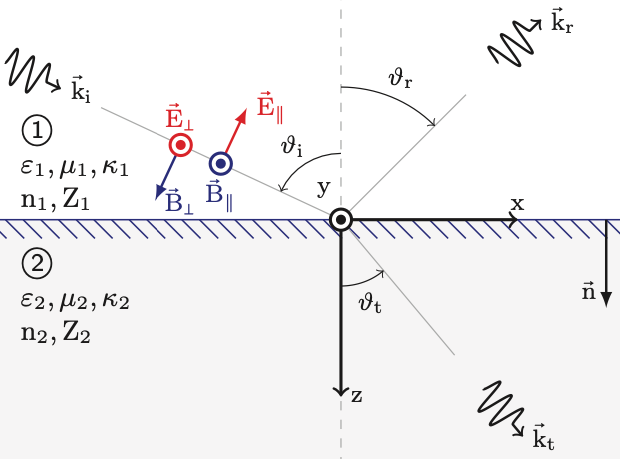
\includegraphics[width=.38\columnwidth]{ref-brech-uebersicht.png}
    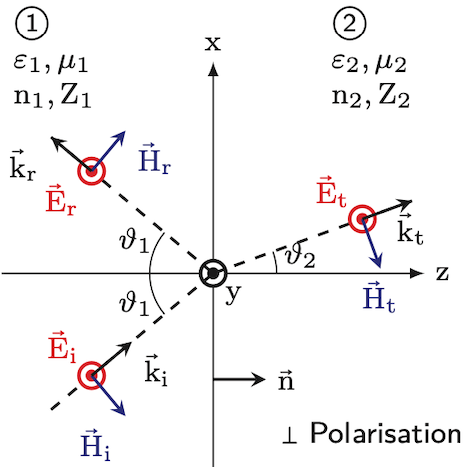
\includegraphics[width=.26\columnwidth]{ref-brech-senk-pol.png}
    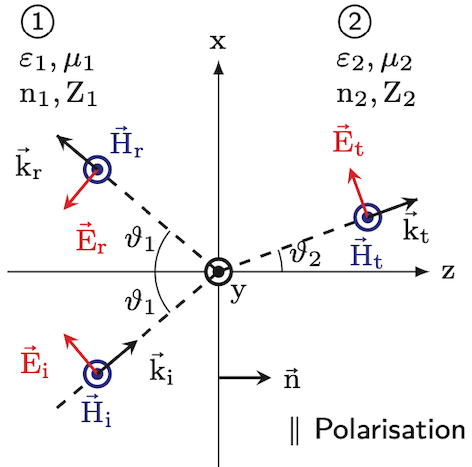
\includegraphics[width=.26\columnwidth]{ref-brech-par-pol.png}\\
    Reflexionsgesetz: $\vartheta_i=\vartheta_r=\vartheta_1$\\
    Brechungsgesetz (Snellius): $n_1\sin\vartheta_1 = n_2\sin\vartheta_2 \text { mit } \vartheta_2=\vartheta_t$\\
    Reflexions- und Transmissionskoeff.: $\underline{r} = \frac{\efeld[u]_{0r}}{\efeld[u]_{0i}} \qquad \underline{t} = \frac{\efeld[u]_{0t}}{\efeld[u]_{0i}}$ \\
    $\underline{r}_\perp = \frac{Z_2\cos\vartheta_1-Z_1\cos\vartheta_2}{Z_1\cos\vartheta_2+Z_2\cos\vartheta_1} , \, 
    1+\underline{r}_\perp = \underline{t}_\perp = \frac{2 Z_2\cos\vartheta_1}{Z_1\cos\vartheta_2+Z_2\cos\vartheta_1}$\\
    $\underline{r}_\parallel = \frac{Z_1\cos\vartheta_1-Z_2\cos\vartheta_2}{Z_2\cos\vartheta_2+Z_1\cos\vartheta_1},\, \frac{Z_2}{Z_1}\left(1+\underline{r}_\parallel\right) = \underline{t}_\parallel = \frac{2 Z_2\cos\vartheta_1}{Z_2\cos\vartheta_2+Z_1\cos\vartheta_1}$\\
    Übergang Luft - Metall: $\underline{r}_\perp \simeq -1, \, \underline{t}_\perp \simeq 0, \, \underline{r}_\parallel \simeq +1 ,\,\underline{t}_\parallel \simeq 0$\\
    mit $n$:\\
    $\underline{r}_\perp = \frac{n_1\cos\vartheta_1-\frac{\mu_1}{\mu_2} n_2\cos\vartheta_2}{n_1\cos\vartheta_1+\frac{\mu_1}{\mu_2} n_2\cos\vartheta_2},\,
    \underline{t}_\perp = \frac{2 n_1\cos\vartheta_1}{n_1\cos\vartheta_1+\frac{\mu_1}{\mu_2} n_2\cos\vartheta_2}$\\
    $\underline{r}_\parallel = \frac{-n_1\cos\vartheta_2+\frac{\mu_1}{\mu_2} n_2\cos\vartheta_1}{n_1\cos\vartheta_2+\frac{\mu_1}{\mu_2} n_2\cos\vartheta_1},\,
    \underline{t}_\parallel = \frac{2 n_1\cos\vartheta_1}{n_1\cos\vartheta_2+\frac{\mu_1}{\mu_2} n_2\cos\vartheta_1}$\\
    mit $\mu_1=\mu_2$:\\
    $\underline{r}_\perp = \frac{\sin\left(\vartheta_2-\vartheta_1\right)}{\sin\left(\vartheta_1+\vartheta_2\right)}, \, \underline{t}_\perp = \frac{2\sin\vartheta_2\cos\vartheta_1}{\sin\left(\vartheta_1+\vartheta_2\right)}$\\
    $\underline{r}_\parallel = \frac{\tan\left(\vartheta_1-\vartheta_2\right)}{\tan\left(\vartheta_1+\vartheta_2\right)}, \, \underline{t}_\parallel = \frac{2\sin\vartheta_2\cos\vartheta_1}{\sin\left(\vartheta_1+\vartheta_2\right) \cos\left(\vartheta_1-\vartheta_2\right)}$\\
    Brewster-Winkel: $\underline{r}_\parallel = 0$ für $\vartheta_1+\vartheta_2 = \frac{\pi}{2} \Rightarrow \wellenzahl[v]_r \perp \wellenzahl[v]_t, \, \tan\vartheta_1=\frac{n_2}{n_1}$\\
    Totalreflexion ($n_1 > n_2$): $\sin\vartheta_{\text{1G}} = \frac{n_2}{n_1}$\\
    Feld im Medium 2 bei Totalreflexion:\\
    $\efeld[uv]_t = t \efeld[u]_{0i} \euler^{-\alpha z} \euler^{\komplex\left(\omega t - \beta x \right)}\einheitsvek{E_t} $ evaneszenter Mode\\
    $\poyvec[uv] = \frac{1}{2 Z_2 k_2} \left|t \efeld[u]_{0i} \right|^2 \euler^{-2\alpha z}\left( \beta \einheitsvek{x} +\komplex \alpha \einheitsvek{z}\right)$\\
    $\alpha = \wellenzahl_2 \sqrt{\left(\frac{n_1}{n_2}\right)^2 \sin^2\vartheta_1-1},\, \beta = \wellenzahl_2 \frac{n_1}{n_2} \sin\vartheta_1$
  \end{minipage}
};
%------------ EM-Wellen: Relexion und Brechung ---------------------
\node[allgtitle, right=10pt] at (box.north west) {EM-Wellen: Reflexion und Brechung};
\end{tikzpicture}


%------------ Retardierte Greensche Funktion und Potentiale ---------------
\begin{tikzpicture}
\node [allgbox] (box){%
  \begin{minipage}{0.3\textwidth}
    $G_{\text{ret}}(\ortsvektor[v]-\ortsvektor[vs], t - t') = \frac{\delta(t'-t_{\text{ret}})}{4\pi |\ortsvektor[v]-\ortsvektor[vs]|}, \, t_{\text{ret}} = t - \frac{|\ortsvektor[v]-\ortsvektor[vs]|}{\geschw_c}$\\
    In Lorenz-Eichung:\\
    $\elpotential (\ortsvektor[v], t) = \frac{1}{4\pi\varepsilon} \iiint_V \frac{\laddichte{V}\left(\ortsvektor[vs], t-t_{\text{ret}}\right)}{|\ortsvektor[v]-\ortsvektor[vs]|} \upd^3\ortsvektor[s]$\\
    $\magvekpot[v] (\ortsvektor[v], t) = \frac{\mu}{4\pi} \iiint_V \frac{\elstromdichte[v]\left(\ortsvektor[vs], t-t_{\text{ret}}\right)}{|\ortsvektor[v]-\ortsvektor[vs]|} \upd^3\ortsvektor[s]$\\
    Lsg. außerhalb Quellgebiet, harm. Anregung:\\
    $\magvekpot[uv] (\ortsvektor[v]) = \frac{\mu}{4\pi} \iiint_V \frac{\euler^{-\komplex \wellenzahl |\ortsvektor[v]-\ortsvektor[vs]|}}{|\ortsvektor[v]-\ortsvektor[vs]|} \elstromdichte[uv](\ortsvektor[vs]) \upd^3 \ortsvektor[s]\to \text{Nah- und Fernzone}$
  \end{minipage}
};
%------------ Retardierte Greensche Funktion und Potentiale ---------------------
\node[allgtitle, right=10pt] at (box.north west) {Retardierte Greensche Funktion und Potentiale};
\end{tikzpicture}

%------------ Linearantennen ---------------
\begin{tikzpicture}
\node [allgbox] (box){%
  \begin{minipage}{0.3\textwidth}
    LE, harm. Anregung, dünner Leiter, Länge $\ell$, z.B. $z$-Richtung:\\
    $\elstromdichte[uv](\ortsvektor[vs]) \upd^3 \ortsvektor[s] = \underline{I}(\ortsvektor[vs])\einheitsvek{z}\upd z^\prime$\\
    $\magvekpot[uv](\ortsvektor[v]) = \frac{\mu}{4\pi} \int_{-\nicefrac{\ell}{2}}^{\nicefrac{\ell}{2}} \frac{\euler^{-\komplex\wellenzahl |\ortsvektor[v]-\ortsvektor[vs]|}}{|\ortsvektor[v]-\ortsvektor[vs]|} \underline{I}(\ortsvektor[vs])\einheitsvek{z}\upd z^\prime$\\
    Allg.: $\upd\magfeld[uv](\ortsvektor[v]) = \frac{1}{4\pi} \underline{I}(\ortsvektor[vs]) \left( \upd\ortsvektor[vs] \times \frac{\ortsvektor[v]-\ortsvektor[vs]}{|\ortsvektor[v]-\ortsvektor[vs]|} \right) \left(\frac{1}{|\ortsvektor[v]-\ortsvektor[vs]|} +\komplex\wellenzahl \right) \frac{\euler^{-\komplex\wellenzahl |\ortsvektor[v]-\ortsvektor[vs]|}}{|\ortsvektor[v]-\ortsvektor[vs]|}$\\
    Fernfeld: $\upd\magfeld[uv](\ortsvektor[v]) = \frac{\komplex\wellenzahl}{4\pi} \underline{I}(\ortsvektor[vs]) \left( \upd\ortsvektor[vs] \times \frac{\ortsvektor[v]}{\ortsvektor} \right) \frac{\euler^{-\komplex\wellenzahl \ortsvektor}}{\ortsvektor} \euler^{\komplex\wellenzahl \frac{\ortsvektor[v]\cdot \ortsvektor[vs]}{\ortsvektor}}$
  \end{minipage}
};
%------------ Linearantennen ---------------------
\node[allgtitle, right=10pt] at (box.north west) {Linearantennen};
\end{tikzpicture}


\end{multicols*}

\newpage

\begin{multicols*}{3}[\textbf{TET Formelsammlung (Prof. H.G. Krauthäuser, TU Dresden, CC0 1.0 Universal) \hfill\tetmark\hfill \thepage}]

%------------ Hertzer Dipol ---------------
\begin{tikzpicture}
\node [allgbox] (box){%
  \begin{minipage}{0.3\textwidth}
    $\magvekpot[uv](\ortsvektor[v]) = \frac{\mu}{4\pi} \underline{I} \ell  \frac{\euler^{-\komplex\wellenzahl\ortsvektor}}{\ortsvektor} \einheitsvek{z} = \magvekpot[u]_z \einheitsvek{z}$\\
  in Kugelkoordinaten:\\
  $ \magvekpot[u]_r =  \frac{\mu}{4\pi} \underline{I} \ell  \frac{\euler^{-\komplex\wellenzahl\ortsvektor}}{\ortsvektor} \cos\vartheta,\, \magvekpot[u]_\vartheta =  - \frac{\mu}{4\pi} \underline{I} \ell  \frac{\euler^{-\komplex\wellenzahl\ortsvektor}}{\ortsvektor} \sin\vartheta , \, \magvekpot[u]_\varphi =0$\\
  $\magfeld[uv] = \frac{1}{4\pi} \frac{\omega^2}{\geschw_p^2}\underline{I} \ell  \euler^{-\komplex\wellenzahl\ortsvektor} \sin\vartheta \left[\frac{1}{(\wellenzahl\ortsvektor)^2}+ \frac{\komplex}{\wellenzahl \ortsvektor} \right]\; \einheitsvek{\varphi}$\\
  $ \efeld[uv] = \left\{\frac{1}{2\pi} Z \frac{\omega^2}{\geschw_p^2}\underline{I} \ell  \euler^{-\komplex\wellenzahl\ortsvektor} \cos\vartheta\left[\frac{1}{(\wellenzahl\ortsvektor)^2} - \frac{\komplex}{(\wellenzahl\ortsvektor)^3}\right]\right\} \einheitsvek{r} + $\\
  $\text{\ \ \ \ \ \ } \left\{ \frac{1}{4\pi} Z \frac{\omega^2}{\geschw_p^2}\underline{I} \ell  \euler^{-\komplex\wellenzahl\ortsvektor} \sin\vartheta\left[\frac{\komplex}{\wellenzahl\ortsvektor}  + \frac{1}{(\wellenzahl\ortsvektor)^2} - \frac{\komplex}{(\wellenzahl\ortsvektor)^3} \right] \right\} \einheitsvek{\vartheta}$\\
  Fernfeld $\wellenzahl \ortsvektor \gg 1$:\\
  $ \magfeld[uv]= \magfeld[u]_\varphi \; \einheitsvek{\varphi} = \frac{\komplex}{4\pi} \frac{\omega^2}{\geschw_p^2}\underline{I} \ell  \frac{\euler^{-\komplex\wellenzahl\ortsvektor}}{\wellenzahl\ortsvektor} \sin\vartheta \; \einheitsvek{\varphi}$\\
  $\efeld[uv] = \efeld[u]_\vartheta \; \einheitsvek{\vartheta} = Z\; \magfeld[u]_\varphi \; \einheitsvek{\vartheta}, \, Z=\frac{|\efeld[uv]|}{|\magfeld[uv]|} = \sqrt{\frac{\mu}{\varepsilon}} = \frac{\wellenzahl}{\omega\varepsilon}$\\
  $\poyvec[uv]  = \frac{1}{2} Z \left( \frac{1}{4\pi} \frac{\omega^2}{\geschw_p^2}\frac{|\underline{I}| \ell}{\wellenzahl\ortsvektor} \right)^2 \left(\sin\vartheta\right)^2 \; \einheitsvek{r} = \poyvec_r(r,\vartheta) \; \einheitsvek{r} = \langle \poyvec[v] \rangle$\\
  $ D(\vartheta,\varphi) = \frac{\poyvec_r(r,\vartheta, \varphi)}{P_{\text{iso}}} = \frac{3}{2} \sin^2\vartheta \; ; \; D_{\text{max}} = D(\vartheta=\frac{\pi}{2}) = \frac{3}{2} $
  \end{minipage}
};
%------------ Hertzscher Dipol Header ---------------------
\node[allgtitle, right=10pt] at (box.north west) {Hertzscher Dipol, am Ursprung, in $z$-Richtung};
\end{tikzpicture}


%------------ Zylindrische Wellenleiter ---------------
\begin{tikzpicture}
\node [allgbox] (box){%
  \begin{minipage}{0.3\textwidth}
    Homogene Wellengleichung $\to$ Helmholtz-Gleichung:\\
    $\square \efeld[uv](\ortsvektor[v], t) = \left(\laplace - \varepsilon\mu\frac{\d^2}{\d t^2}\right) \efeld[uv] (\ortsvektor[v], t) = \vec{0} \rightarrow  \left(\laplace + \varepsilon\mu\omega^2\right) \efeld[uv](\ortsvektor[v]) =\vec{0}$\\
    $\square \magflussd[uv](\ortsvektor[v], t) = \left(\laplace - \varepsilon\mu\frac{\d^2}{\d t^2}\right) \magflussd[uv] (\ortsvektor[v], t) = \vec{0} \rightarrow  \left(\laplace + \varepsilon\mu\omega^2\right) \magflussd[uv](\ortsvektor[v]) =\vec{0}$\\
    $\einheitsvek{z} \cdot \left(\rotation_t \efeld[uv]_t\right) = -\komplex\omega\magflussd[u]_z, \ \gradient_t \efeld[u]_{z} - \frac{\partial}{\partial z}\efeld[uv]_t = -\komplex\omega \einheitsvek{z}\times \magflussd[uv]_t$\\
    $ \einheitsvek{z} \cdot \left(\rotation_t \magflussd[uv]_t\right) = \komplex\omega\varepsilon\mu\efeld[u]_z ,\  \gradient_t \magflussd[u]_{z} - \frac{\partial}{\partial z}\magflussd[uv]_t = \komplex\omega\varepsilon\mu \einheitsvek{z}\times \efeld[uv]_t$\\
    entkoppelt ('-': vor; '+': rück); $\gamma^2 = \omega^2\varepsilon\mu - \wellenzahl^2$\\
    $\gamma^2 \efeld[uv]_t = \komplex \left[ \mp \wellenzahl\, \gradient_t \efeld[u]_{z} + \omega  \einheitsvek{z}\times\gradient_t \magflussd[u]_{z}\right]$\\
    $\gamma^2 \magflussd[uv]_t = \komplex \left[ \mp \wellenzahl\, \gradient_t \magflussd[u]_{z} - \omega\varepsilon\mu  \einheitsvek{z}\times\gradient_t \efeld[u]_{z}\right]$\\
    TEM: $\efeld[u]_{z} = \magflussd[u]_{z} = \vec{0}\to \gamma^2=0$, oder triviale Lösung\\
    \text{\phantom{TEM: }}$\efeld[uv] =\efeld[uv]_t= -\gradient\elpotential$ mit $\laplace_t \elpotential = \laplace_t \elpotential_t = 0$\\
    \text{\phantom{TEM: }}$ \magflussd[uv] = \pm \sqrt{\varepsilon\mu}\, \einheitsvek{z}\times\efeld[uv] \quad \text{ ('+' = hin)}$\\
    \text{\phantom{TEM: }}$\magfeld[uv] = \pm \frac{1}{Z}\, \einheitsvek{z}\times\efeld[uv] \quad\text{ ('+' = hin)}$\\
    TM/TE: $\magflussd[u]_z = 0$ bzw. $\efeld[u]_z = 0$, $\gamma^2\ne 0$\\
    \text{\phantom{TM/TE: }}$\left(\laplace_t + \gamma^2\right) \efeld[u]_z =  0$ bzw. $\left(\laplace_t + \gamma^2\right) \magfeld[u]_z =  0$ mit Randbed.\\
    \text{\phantom{TM/TE: }}Dispersionsrelation: $\wellenzahl_\lambda=\sqrt{\mu\varepsilon}\sqrt{\omega^2-\omega_\lambda^2} \text{ mit } \omega_\lambda=\frac{\gamma_\lambda}{\sqrt{\mu\varepsilon}}$
  \end{minipage}
};
%------------ Zylinderische Wellenleiter Header ---------------------
\node[allgtitle, right=10pt] at (box.north west) {Zylindrische Wellenleiter, $z$-Richtung, $\kappa = \infty$, harmonisch};
\end{tikzpicture}


\newcolumn

%------------ Klassische Leitungstheorie ---------------
\begin{tikzpicture}
\node [allgbox] (box){%
  \begin{minipage}{0.3\textwidth}
    Im Querschnitt:\\
    $\elpotential=\elpotential(x,y), \laplace\elpotential(x,y) = 0, \,\elpotential = 0 \text{ bzw. } \elpotential = \spannung(z) \text{ auf Leiter}$\\
    Telegraphengleichungen:\\
    $\frac{\d \spannung[u](z)}{\d z} + \left(R^\prime + \komplex\omega L^\prime\right) \elstrom[u](z)= 0, \; L^\prime = \frac{\mu\int_C\gradient\elpotential \cdot \upd \vec{s}}{\oint_{O(A)} \left(\einheitsvek{z}\times\gradient\elpotential\right) \cdot \upd\vec{s}}$\\
    $\frac{\d \elstrom[u](z)}{\d z} +\left(G^\prime + \komplex\omega C^\prime\right) \spannung[u](z)  = 0,\; C^\prime = \frac{\varepsilon\oint_{O(A)}\left(\einheitsvek{z}\times \gradient\elpotential\right) \cdot \upd \vec{s}}{\int_C \gradient\elpotential\cdot\upd\vec{s}}$\\
    $\geschw_p = \frac{1}{\sqrt{L^\prime C^\prime}}=\frac{1}{\sqrt{\varepsilon\mu}}$\\
    entkoppelt: $ \frac{\d^2 \spannung[u](z)}{\d z^2} - Z^\prime Y^\prime \spannung[u](z) = 0,\; \frac{\d^2 \elstrom[u](z)}{\d z^2} - Z^\prime Y^\prime \elstrom[u](z) = 0 $\\
     Ausbreitungskonstante: $\gamma = \sqrt{Z^\prime Y^\prime} = \sqrt{\left(R^\prime + \komplex\omega L^\prime\right) \left(G^\prime + \komplex\omega C^\prime\right)}$\\
    Lösungen: $\spannung[u](z) = u_1 \euler^{-\gamma z} + u_2 \euler^{+\gamma z}$ Randbed. beachten\\
    \text{\phantom{Lösungen: }}$\elstrom[u](z) = \frac{1}{Z_L} \left( u_1 \euler^{-\gamma z} - u_2 \euler^{+\gamma z}\right)$\\
    Leitungswellenwiderstand: $Z_L= \frac{Z^\prime}{\gamma} = \sqrt{\frac{Z^\prime}{Y^\prime}} = \sqrt{\frac{R^\prime + \komplex\omega L^\prime}{G^\prime + \komplex\omega C^\prime}}$
  \end{minipage}
};
%------------ Klassische Leitungstheorie Header ---------------------
\node[allgtitle, right=10pt] at (box.north west) {Klassische Leitungstheorie};
\end{tikzpicture}



\end{multicols*}


\end{document}